\documentclass[twoside]{book}

% Packages required by doxygen
\usepackage{fixltx2e}
\usepackage{calc}
\usepackage{doxygen}
\usepackage[export]{adjustbox} % also loads graphicx
\usepackage{graphicx}
\usepackage[utf8]{inputenc}
\usepackage{makeidx}
\usepackage{multicol}
\usepackage{multirow}
\PassOptionsToPackage{warn}{textcomp}
\usepackage{textcomp}
\usepackage[nointegrals]{wasysym}
\usepackage[table]{xcolor}

% NLS support packages
\usepackage[T2A]{fontenc}
\usepackage[russian]{babel}

% Font selection
\usepackage[T1]{fontenc}
\usepackage[scaled=.90]{helvet}
\usepackage{courier}
\usepackage{amssymb}
\usepackage{sectsty}
\renewcommand{\familydefault}{\sfdefault}
\allsectionsfont{%
  \fontseries{bc}\selectfont%
  \color{darkgray}%
}
\renewcommand{\DoxyLabelFont}{%
  \fontseries{bc}\selectfont%
  \color{darkgray}%
}
\newcommand{\+}{\discretionary{\mbox{\scriptsize$\hookleftarrow$}}{}{}}

% Page & text layout
\usepackage{geometry}
\geometry{%
  a4paper,%
  top=2.5cm,%
  bottom=2.5cm,%
  left=2.5cm,%
  right=2.5cm%
}
\tolerance=750
\hfuzz=15pt
\hbadness=750
\setlength{\emergencystretch}{15pt}
\setlength{\parindent}{0cm}
\setlength{\parskip}{3ex plus 2ex minus 2ex}
\makeatletter
\renewcommand{\paragraph}{%
  \@startsection{paragraph}{4}{0ex}{-1.0ex}{1.0ex}{%
    \normalfont\normalsize\bfseries\SS@parafont%
  }%
}
\renewcommand{\subparagraph}{%
  \@startsection{subparagraph}{5}{0ex}{-1.0ex}{1.0ex}{%
    \normalfont\normalsize\bfseries\SS@subparafont%
  }%
}
\makeatother

% Headers & footers
\usepackage{fancyhdr}
\pagestyle{fancyplain}
\fancyhead[LE]{\fancyplain{}{\bfseries\thepage}}
\fancyhead[CE]{\fancyplain{}{}}
\fancyhead[RE]{\fancyplain{}{\bfseries\leftmark}}
\fancyhead[LO]{\fancyplain{}{\bfseries\rightmark}}
\fancyhead[CO]{\fancyplain{}{}}
\fancyhead[RO]{\fancyplain{}{\bfseries\thepage}}
\fancyfoot[LE]{\fancyplain{}{}}
\fancyfoot[CE]{\fancyplain{}{}}
\fancyfoot[RE]{\fancyplain{}{\bfseries\scriptsize Создано системой Doxygen }}
\fancyfoot[LO]{\fancyplain{}{\bfseries\scriptsize Создано системой Doxygen }}
\fancyfoot[CO]{\fancyplain{}{}}
\fancyfoot[RO]{\fancyplain{}{}}
\renewcommand{\footrulewidth}{0.4pt}
\renewcommand{\chaptermark}[1]{%
  \markboth{#1}{}%
}
\renewcommand{\sectionmark}[1]{%
  \markright{\thesection\ #1}%
}

% Indices & bibliography
\usepackage{natbib}
\usepackage[titles]{tocloft}
\setcounter{tocdepth}{3}
\setcounter{secnumdepth}{5}
\makeindex

% Hyperlinks (required, but should be loaded last)
\usepackage{ifpdf}
\ifpdf
  \usepackage[pdftex,pagebackref=true]{hyperref}
\else
  \usepackage[ps2pdf,pagebackref=true]{hyperref}
\fi
\hypersetup{%
  colorlinks=true,%
  linkcolor=blue,%
  citecolor=blue,%
  unicode%
}

% Custom commands
\newcommand{\clearemptydoublepage}{%
  \newpage{\pagestyle{empty}\cleardoublepage}%
}

\usepackage{caption}
\captionsetup{labelsep=space,justification=centering,font={bf},singlelinecheck=off,skip=4pt,position=top}

%===== C O N T E N T S =====

\begin{document}

% Titlepage & ToC
\hypersetup{pageanchor=false,
             bookmarksnumbered=true,
             pdfencoding=unicode
            }
\pagenumbering{alph}
\begin{titlepage}
\vspace*{7cm}
\begin{center}%
{\Large Game-\/2D }\\
\vspace*{1cm}
{\large Создано системой Doxygen 1.8.13}\\
\end{center}
\end{titlepage}
\clearemptydoublepage
\pagenumbering{roman}
\tableofcontents
\clearemptydoublepage
\pagenumbering{arabic}
\hypersetup{pageanchor=true}

%--- Begin generated contents ---
\chapter{Алфавитный указатель пространств имен}
\section{Пакеты}
Полный список документированных пакетов.\begin{DoxyCompactList}
\item\contentsline{section}{\hyperlink{namespace_game}{Game} }{\pageref{namespace_game}}{}
\item\contentsline{section}{\hyperlink{namespace_game_1_1_enums}{Game.\+Enums} }{\pageref{namespace_game_1_1_enums}}{}
\item\contentsline{section}{\hyperlink{namespace_game_1_1_extension}{Game.\+Extension} }{\pageref{namespace_game_1_1_extension}}{}
\item\contentsline{section}{\hyperlink{namespace_game_1_1_models}{Game.\+Models} }{\pageref{namespace_game_1_1_models}}{}
\item\contentsline{section}{\hyperlink{namespace_game_1_1_properties}{Game.\+Properties} }{\pageref{namespace_game_1_1_properties}}{}
\end{DoxyCompactList}

\chapter{Иерархический список классов}
\section{Иерархия классов}
Иерархия классов.\begin{DoxyCompactList}
\item Form\begin{DoxyCompactList}
\item \contentsline{section}{Game.\+Form1}{\pageref{class_game_1_1_form1}}{}
\end{DoxyCompactList}
\item \contentsline{section}{Game.\+Extension.\+Game\+Control}{\pageref{class_game_1_1_extension_1_1_game_control}}{}
\item \contentsline{section}{Game.\+Extension.\+Game\+Rendering}{\pageref{class_game_1_1_extension_1_1_game_rendering}}{}
\item \contentsline{section}{Game.\+Extension.\+Game\+Textures}{\pageref{class_game_1_1_extension_1_1_game_textures}}{}
\item \contentsline{section}{Game.\+Models.\+Net}{\pageref{class_game_1_1_models_1_1_net}}{}
\item \contentsline{section}{Game.\+Models.\+Path\+Node}{\pageref{class_game_1_1_models_1_1_path_node}}{}
\item \contentsline{section}{Game.\+Program}{\pageref{class_game_1_1_program}}{}
\item \contentsline{section}{Game.\+Extension.\+Work\+With\+Time}{\pageref{class_game_1_1_extension_1_1_work_with_time}}{}
\end{DoxyCompactList}

\chapter{Алфавитный указатель классов}
\section{Классы}
Классы с их кратким описанием.\begin{DoxyCompactList}
\item\contentsline{section}{\hyperlink{class_game_1_1_form1}{Game.\+Form1} \\*Класс формы, на которой происходит отображение всех объектов }{\pageref{class_game_1_1_form1}}{}
\item\contentsline{section}{\hyperlink{class_game_1_1_extension_1_1_game_control}{Game.\+Extension.\+Game\+Control} \\*Класс расширения Алгоритм нахождения кратчайшего расстояния между двумя точками — A$\ast$ }{\pageref{class_game_1_1_extension_1_1_game_control}}{}
\item\contentsline{section}{\hyperlink{class_game_1_1_extension_1_1_game_rendering}{Game.\+Extension.\+Game\+Rendering} \\*Класс расширения Отрисовка объектов }{\pageref{class_game_1_1_extension_1_1_game_rendering}}{}
\item\contentsline{section}{\hyperlink{class_game_1_1_extension_1_1_game_textures}{Game.\+Extension.\+Game\+Textures} \\*Класс расширения Работа с текстурами (загрузка) }{\pageref{class_game_1_1_extension_1_1_game_textures}}{}
\item\contentsline{section}{\hyperlink{class_game_1_1_models_1_1_net}{Game.\+Models.\+Net} \\*Класс сетки, на котоой отображаются объекты }{\pageref{class_game_1_1_models_1_1_net}}{}
\item\contentsline{section}{\hyperlink{class_game_1_1_models_1_1_path_node}{Game.\+Models.\+Path\+Node} \\*Структура, используемая в алгоритме A$\ast$ }{\pageref{class_game_1_1_models_1_1_path_node}}{}
\item\contentsline{section}{\hyperlink{class_game_1_1_program}{Game.\+Program} }{\pageref{class_game_1_1_program}}{}
\item\contentsline{section}{\hyperlink{class_game_1_1_extension_1_1_work_with_time}{Game.\+Extension.\+Work\+With\+Time} \\*Класс расширения Работа со временем }{\pageref{class_game_1_1_extension_1_1_work_with_time}}{}
\end{DoxyCompactList}

\chapter{Пространства имен}
\hypertarget{namespace_game}{}\section{Пространство имен Game}
\label{namespace_game}\index{Game@{Game}}
\subsection*{Пространства имен}
\begin{DoxyCompactItemize}
\end{DoxyCompactItemize}
\subsection*{Классы}
\begin{DoxyCompactItemize}
\item 
class \hyperlink{class_game_1_1_form1}{Form1}
\begin{DoxyCompactList}\small\item\em Класс формы, на которой происходит отображение всех объектов \end{DoxyCompactList}\item 
class \hyperlink{class_game_1_1_program}{Program}
\end{DoxyCompactItemize}

\hypertarget{namespace_game_1_1_enums}{}\section{Пространство имен Game.\+Enums}
\label{namespace_game_1_1_enums}\index{Game.\+Enums@{Game.\+Enums}}
\subsection*{Перечисления}
\begin{DoxyCompactItemize}
\item 
enum \hyperlink{namespace_game_1_1_enums_afecfa7946d85e70582de0c788cc185bd}{Direction} \{ \newline
\hyperlink{namespace_game_1_1_enums_afecfa7946d85e70582de0c788cc185bdafbaedde498cdead4f2780217646e9ba1}{Direction.\+UP}, 
\hyperlink{namespace_game_1_1_enums_afecfa7946d85e70582de0c788cc185bdac4e0e4e3118472beeb2ae75827450f1f}{Direction.\+D\+O\+WN}, 
\hyperlink{namespace_game_1_1_enums_afecfa7946d85e70582de0c788cc185bda684d325a7303f52e64011467ff5c5758}{Direction.\+L\+E\+FT}, 
\hyperlink{namespace_game_1_1_enums_afecfa7946d85e70582de0c788cc185bda21507b40c80068eda19865706fdc2403}{Direction.\+R\+I\+G\+HT}, 
\newline
\hyperlink{namespace_game_1_1_enums_afecfa7946d85e70582de0c788cc185bdafaee13016b273769adaa8e118bf510d6}{Direction.\+Upper\+Right\+Corner}, 
\hyperlink{namespace_game_1_1_enums_afecfa7946d85e70582de0c788cc185bda03570470bad94692ce93e32700d2e1cb}{Direction.\+O\+T\+H\+ER}
 \}\begin{DoxyCompactList}\small\item\em Направление \end{DoxyCompactList}
\item 
enum \hyperlink{namespace_game_1_1_enums_a2d1ea7762a7b4609383b4b578d1c4a60}{Textures} \{ \newline
\hyperlink{namespace_game_1_1_enums_a2d1ea7762a7b4609383b4b578d1c4a60ae1e4c8c9ccd9fc39c391da4bcd093fb2}{Textures.\+Block} = 0, 
\hyperlink{namespace_game_1_1_enums_a2d1ea7762a7b4609383b4b578d1c4a60aa0544b6900b52d329c015b250c112438}{Textures.\+Transparent\+Character} = 1, 
\hyperlink{namespace_game_1_1_enums_a2d1ea7762a7b4609383b4b578d1c4a60a933ae9c7efe484b7f6acde743180f10e}{Textures.\+Current\+Charactert} = 2, 
\hyperlink{namespace_game_1_1_enums_a2d1ea7762a7b4609383b4b578d1c4a60a90e78b5932e9d454180ca939b27863be}{Textures.\+Toarch} = 3, 
\newline
\hyperlink{namespace_game_1_1_enums_a2d1ea7762a7b4609383b4b578d1c4a60ad9dbe6b81249a8334f10e076154537d3}{Textures.\+Grass\+Day} = 4, 
\hyperlink{namespace_game_1_1_enums_a2d1ea7762a7b4609383b4b578d1c4a60af20f7ae1531e4dc39cefc9d0c6cd819a}{Textures.\+Grass\+Night} = 5
 \}\begin{DoxyCompactList}\small\item\em Обозначния текстур \end{DoxyCompactList}
\item 
enum \hyperlink{namespace_game_1_1_enums_ab6782702f41f926eb2b923ee03a88069}{Type\+Of\+Cell} \{ \newline
\hyperlink{namespace_game_1_1_enums_ab6782702f41f926eb2b923ee03a88069ab3e25d19bfd437de6063953f0f4ac6ac}{Type\+Of\+Cell.\+Block1}, 
\hyperlink{namespace_game_1_1_enums_ab6782702f41f926eb2b923ee03a88069a3fbe9f2beae8654b86e2d9570f63d4e2}{Type\+Of\+Cell.\+Block2}, 
\hyperlink{namespace_game_1_1_enums_ab6782702f41f926eb2b923ee03a88069a5331717d33d4e634fd3c5ec209f475d2}{Type\+Of\+Cell.\+Lamp}, 
\hyperlink{namespace_game_1_1_enums_ab6782702f41f926eb2b923ee03a88069ab24ce0cd392a5b0b8dedc66c25213594}{Type\+Of\+Cell.\+Free}, 
\newline
\hyperlink{namespace_game_1_1_enums_ab6782702f41f926eb2b923ee03a88069aa20ddccbb6f808ec42cd66323e6c6061}{Type\+Of\+Cell.\+Finish}
 \}\begin{DoxyCompactList}\small\item\em Тип клетки \end{DoxyCompactList}
\end{DoxyCompactItemize}


\subsection{Перечисления}
\mbox{\Hypertarget{namespace_game_1_1_enums_afecfa7946d85e70582de0c788cc185bd}\label{namespace_game_1_1_enums_afecfa7946d85e70582de0c788cc185bd}} 
\index{Game\+::\+Enums@{Game\+::\+Enums}!Direction@{Direction}}
\index{Direction@{Direction}!Game\+::\+Enums@{Game\+::\+Enums}}
\subsubsection{\texorpdfstring{Direction}{Direction}}
{\footnotesize\ttfamily enum \hyperlink{namespace_game_1_1_enums_afecfa7946d85e70582de0c788cc185bd}{Game.\+Enums.\+Direction}\hspace{0.3cm}{\ttfamily [strong]}}



Направление 

\begin{DoxyEnumFields}{Элементы перечислений}
\raisebox{\heightof{T}}[0pt][0pt]{\index{UP@{UP}!Game\+::\+Enums@{Game\+::\+Enums}}\index{Game\+::\+Enums@{Game\+::\+Enums}!UP@{UP}}}\mbox{\Hypertarget{namespace_game_1_1_enums_afecfa7946d85e70582de0c788cc185bdafbaedde498cdead4f2780217646e9ba1}\label{namespace_game_1_1_enums_afecfa7946d85e70582de0c788cc185bdafbaedde498cdead4f2780217646e9ba1}} 
UP&Вверх \\
\hline

\raisebox{\heightof{T}}[0pt][0pt]{\index{D\+O\+WN@{D\+O\+WN}!Game\+::\+Enums@{Game\+::\+Enums}}\index{Game\+::\+Enums@{Game\+::\+Enums}!D\+O\+WN@{D\+O\+WN}}}\mbox{\Hypertarget{namespace_game_1_1_enums_afecfa7946d85e70582de0c788cc185bdac4e0e4e3118472beeb2ae75827450f1f}\label{namespace_game_1_1_enums_afecfa7946d85e70582de0c788cc185bdac4e0e4e3118472beeb2ae75827450f1f}} 
D\+O\+WN&Вниз \\
\hline

\raisebox{\heightof{T}}[0pt][0pt]{\index{L\+E\+FT@{L\+E\+FT}!Game\+::\+Enums@{Game\+::\+Enums}}\index{Game\+::\+Enums@{Game\+::\+Enums}!L\+E\+FT@{L\+E\+FT}}}\mbox{\Hypertarget{namespace_game_1_1_enums_afecfa7946d85e70582de0c788cc185bda684d325a7303f52e64011467ff5c5758}\label{namespace_game_1_1_enums_afecfa7946d85e70582de0c788cc185bda684d325a7303f52e64011467ff5c5758}} 
L\+E\+FT&Вправо \\
\hline

\raisebox{\heightof{T}}[0pt][0pt]{\index{R\+I\+G\+HT@{R\+I\+G\+HT}!Game\+::\+Enums@{Game\+::\+Enums}}\index{Game\+::\+Enums@{Game\+::\+Enums}!R\+I\+G\+HT@{R\+I\+G\+HT}}}\mbox{\Hypertarget{namespace_game_1_1_enums_afecfa7946d85e70582de0c788cc185bda21507b40c80068eda19865706fdc2403}\label{namespace_game_1_1_enums_afecfa7946d85e70582de0c788cc185bda21507b40c80068eda19865706fdc2403}} 
R\+I\+G\+HT&Влево \\
\hline

\raisebox{\heightof{T}}[0pt][0pt]{\index{Upper\+Right\+Corner@{Upper\+Right\+Corner}!Game\+::\+Enums@{Game\+::\+Enums}}\index{Game\+::\+Enums@{Game\+::\+Enums}!Upper\+Right\+Corner@{Upper\+Right\+Corner}}}\mbox{\Hypertarget{namespace_game_1_1_enums_afecfa7946d85e70582de0c788cc185bdafaee13016b273769adaa8e118bf510d6}\label{namespace_game_1_1_enums_afecfa7946d85e70582de0c788cc185bdafaee13016b273769adaa8e118bf510d6}} 
Upper\+Right\+Corner&Верхний правый угол \\
\hline

\raisebox{\heightof{T}}[0pt][0pt]{\index{O\+T\+H\+ER@{O\+T\+H\+ER}!Game\+::\+Enums@{Game\+::\+Enums}}\index{Game\+::\+Enums@{Game\+::\+Enums}!O\+T\+H\+ER@{O\+T\+H\+ER}}}\mbox{\Hypertarget{namespace_game_1_1_enums_afecfa7946d85e70582de0c788cc185bda03570470bad94692ce93e32700d2e1cb}\label{namespace_game_1_1_enums_afecfa7946d85e70582de0c788cc185bda03570470bad94692ce93e32700d2e1cb}} 
O\+T\+H\+ER&Остальные направления \\
\hline

\end{DoxyEnumFields}
\mbox{\Hypertarget{namespace_game_1_1_enums_a2d1ea7762a7b4609383b4b578d1c4a60}\label{namespace_game_1_1_enums_a2d1ea7762a7b4609383b4b578d1c4a60}} 
\index{Game\+::\+Enums@{Game\+::\+Enums}!Textures@{Textures}}
\index{Textures@{Textures}!Game\+::\+Enums@{Game\+::\+Enums}}
\subsubsection{\texorpdfstring{Textures}{Textures}}
{\footnotesize\ttfamily enum \hyperlink{namespace_game_1_1_enums_a2d1ea7762a7b4609383b4b578d1c4a60}{Game.\+Enums.\+Textures}\hspace{0.3cm}{\ttfamily [strong]}}



Обозначния текстур 

\begin{DoxyEnumFields}{Элементы перечислений}
\raisebox{\heightof{T}}[0pt][0pt]{\index{Block@{Block}!Game\+::\+Enums@{Game\+::\+Enums}}\index{Game\+::\+Enums@{Game\+::\+Enums}!Block@{Block}}}\mbox{\Hypertarget{namespace_game_1_1_enums_a2d1ea7762a7b4609383b4b578d1c4a60ae1e4c8c9ccd9fc39c391da4bcd093fb2}\label{namespace_game_1_1_enums_a2d1ea7762a7b4609383b4b578d1c4a60ae1e4c8c9ccd9fc39c391da4bcd093fb2}} 
Block&Препятствие \\
\hline

\raisebox{\heightof{T}}[0pt][0pt]{\index{Transparent\+Character@{Transparent\+Character}!Game\+::\+Enums@{Game\+::\+Enums}}\index{Game\+::\+Enums@{Game\+::\+Enums}!Transparent\+Character@{Transparent\+Character}}}\mbox{\Hypertarget{namespace_game_1_1_enums_a2d1ea7762a7b4609383b4b578d1c4a60aa0544b6900b52d329c015b250c112438}\label{namespace_game_1_1_enums_a2d1ea7762a7b4609383b4b578d1c4a60aa0544b6900b52d329c015b250c112438}} 
Transparent\+Character&Персонаж прозрачный \\
\hline

\raisebox{\heightof{T}}[0pt][0pt]{\index{Current\+Charactert@{Current\+Charactert}!Game\+::\+Enums@{Game\+::\+Enums}}\index{Game\+::\+Enums@{Game\+::\+Enums}!Current\+Charactert@{Current\+Charactert}}}\mbox{\Hypertarget{namespace_game_1_1_enums_a2d1ea7762a7b4609383b4b578d1c4a60a933ae9c7efe484b7f6acde743180f10e}\label{namespace_game_1_1_enums_a2d1ea7762a7b4609383b4b578d1c4a60a933ae9c7efe484b7f6acde743180f10e}} 
Current\+Charactert&Персонаж текущий \\
\hline

\raisebox{\heightof{T}}[0pt][0pt]{\index{Toarch@{Toarch}!Game\+::\+Enums@{Game\+::\+Enums}}\index{Game\+::\+Enums@{Game\+::\+Enums}!Toarch@{Toarch}}}\mbox{\Hypertarget{namespace_game_1_1_enums_a2d1ea7762a7b4609383b4b578d1c4a60a90e78b5932e9d454180ca939b27863be}\label{namespace_game_1_1_enums_a2d1ea7762a7b4609383b4b578d1c4a60a90e78b5932e9d454180ca939b27863be}} 
Toarch&Факел \\
\hline

\raisebox{\heightof{T}}[0pt][0pt]{\index{Grass\+Day@{Grass\+Day}!Game\+::\+Enums@{Game\+::\+Enums}}\index{Game\+::\+Enums@{Game\+::\+Enums}!Grass\+Day@{Grass\+Day}}}\mbox{\Hypertarget{namespace_game_1_1_enums_a2d1ea7762a7b4609383b4b578d1c4a60ad9dbe6b81249a8334f10e076154537d3}\label{namespace_game_1_1_enums_a2d1ea7762a7b4609383b4b578d1c4a60ad9dbe6b81249a8334f10e076154537d3}} 
Grass\+Day&Трава Днем \\
\hline

\raisebox{\heightof{T}}[0pt][0pt]{\index{Grass\+Night@{Grass\+Night}!Game\+::\+Enums@{Game\+::\+Enums}}\index{Game\+::\+Enums@{Game\+::\+Enums}!Grass\+Night@{Grass\+Night}}}\mbox{\Hypertarget{namespace_game_1_1_enums_a2d1ea7762a7b4609383b4b578d1c4a60af20f7ae1531e4dc39cefc9d0c6cd819a}\label{namespace_game_1_1_enums_a2d1ea7762a7b4609383b4b578d1c4a60af20f7ae1531e4dc39cefc9d0c6cd819a}} 
Grass\+Night&Трава Ночью \\
\hline

\end{DoxyEnumFields}
\mbox{\Hypertarget{namespace_game_1_1_enums_ab6782702f41f926eb2b923ee03a88069}\label{namespace_game_1_1_enums_ab6782702f41f926eb2b923ee03a88069}} 
\index{Game\+::\+Enums@{Game\+::\+Enums}!Type\+Of\+Cell@{Type\+Of\+Cell}}
\index{Type\+Of\+Cell@{Type\+Of\+Cell}!Game\+::\+Enums@{Game\+::\+Enums}}
\subsubsection{\texorpdfstring{Type\+Of\+Cell}{TypeOfCell}}
{\footnotesize\ttfamily enum \hyperlink{namespace_game_1_1_enums_ab6782702f41f926eb2b923ee03a88069}{Game.\+Enums.\+Type\+Of\+Cell}\hspace{0.3cm}{\ttfamily [strong]}}



Тип клетки 

\begin{DoxyEnumFields}{Элементы перечислений}
\raisebox{\heightof{T}}[0pt][0pt]{\index{Block1@{Block1}!Game\+::\+Enums@{Game\+::\+Enums}}\index{Game\+::\+Enums@{Game\+::\+Enums}!Block1@{Block1}}}\mbox{\Hypertarget{namespace_game_1_1_enums_ab6782702f41f926eb2b923ee03a88069ab3e25d19bfd437de6063953f0f4ac6ac}\label{namespace_game_1_1_enums_ab6782702f41f926eb2b923ee03a88069ab3e25d19bfd437de6063953f0f4ac6ac}} 
Block1&Препятствие, расположенное по краям карты \\
\hline

\raisebox{\heightof{T}}[0pt][0pt]{\index{Block2@{Block2}!Game\+::\+Enums@{Game\+::\+Enums}}\index{Game\+::\+Enums@{Game\+::\+Enums}!Block2@{Block2}}}\mbox{\Hypertarget{namespace_game_1_1_enums_ab6782702f41f926eb2b923ee03a88069a3fbe9f2beae8654b86e2d9570f63d4e2}\label{namespace_game_1_1_enums_ab6782702f41f926eb2b923ee03a88069a3fbe9f2beae8654b86e2d9570f63d4e2}} 
Block2&Внутренние препятствия карты \\
\hline

\raisebox{\heightof{T}}[0pt][0pt]{\index{Lamp@{Lamp}!Game\+::\+Enums@{Game\+::\+Enums}}\index{Game\+::\+Enums@{Game\+::\+Enums}!Lamp@{Lamp}}}\mbox{\Hypertarget{namespace_game_1_1_enums_ab6782702f41f926eb2b923ee03a88069a5331717d33d4e634fd3c5ec209f475d2}\label{namespace_game_1_1_enums_ab6782702f41f926eb2b923ee03a88069a5331717d33d4e634fd3c5ec209f475d2}} 
Lamp&Факел \\
\hline

\raisebox{\heightof{T}}[0pt][0pt]{\index{Free@{Free}!Game\+::\+Enums@{Game\+::\+Enums}}\index{Game\+::\+Enums@{Game\+::\+Enums}!Free@{Free}}}\mbox{\Hypertarget{namespace_game_1_1_enums_ab6782702f41f926eb2b923ee03a88069ab24ce0cd392a5b0b8dedc66c25213594}\label{namespace_game_1_1_enums_ab6782702f41f926eb2b923ee03a88069ab24ce0cd392a5b0b8dedc66c25213594}} 
Free&Свободная клетка \\
\hline

\raisebox{\heightof{T}}[0pt][0pt]{\index{Finish@{Finish}!Game\+::\+Enums@{Game\+::\+Enums}}\index{Game\+::\+Enums@{Game\+::\+Enums}!Finish@{Finish}}}\mbox{\Hypertarget{namespace_game_1_1_enums_ab6782702f41f926eb2b923ee03a88069aa20ddccbb6f808ec42cd66323e6c6061}\label{namespace_game_1_1_enums_ab6782702f41f926eb2b923ee03a88069aa20ddccbb6f808ec42cd66323e6c6061}} 
Finish&Финишная клетка \\
\hline

\end{DoxyEnumFields}

\hypertarget{namespace_game_1_1_extension}{}\section{Пространство имен Game.\+Extension}
\label{namespace_game_1_1_extension}\index{Game.\+Extension@{Game.\+Extension}}
\subsection*{Классы}
\begin{DoxyCompactItemize}
\item 
class \hyperlink{class_game_1_1_extension_1_1_game_control}{Game\+Control}
\begin{DoxyCompactList}\small\item\em Класс расширения Алгоритм нахождения кратчайшего расстояния между двумя точками — A$\ast$ \end{DoxyCompactList}\item 
class \hyperlink{class_game_1_1_extension_1_1_game_rendering}{Game\+Rendering}
\begin{DoxyCompactList}\small\item\em Класс расширения Отрисовка объектов \end{DoxyCompactList}\item 
class \hyperlink{class_game_1_1_extension_1_1_game_textures}{Game\+Textures}
\begin{DoxyCompactList}\small\item\em Класс расширения Работа с текстурами (загрузка) \end{DoxyCompactList}\item 
class \hyperlink{class_game_1_1_extension_1_1_work_with_time}{Work\+With\+Time}
\begin{DoxyCompactList}\small\item\em Класс расширения Работа со временем \end{DoxyCompactList}\end{DoxyCompactItemize}

\hypertarget{namespace_game_1_1_models}{}\section{Пространство имен Game.\+Models}
\label{namespace_game_1_1_models}\index{Game.\+Models@{Game.\+Models}}
\subsection*{Классы}
\begin{DoxyCompactItemize}
\item 
class \hyperlink{class_game_1_1_models_1_1_net}{Net}
\begin{DoxyCompactList}\small\item\em Класс сетки, на котоой отображаются объекты \end{DoxyCompactList}\item 
class \hyperlink{class_game_1_1_models_1_1_path_node}{Path\+Node}
\begin{DoxyCompactList}\small\item\em Структура, используемая в алгоритме A$\ast$ \end{DoxyCompactList}\end{DoxyCompactItemize}

\hypertarget{namespace_game_1_1_properties}{}\section{Пространство имен Game.\+Properties}
\label{namespace_game_1_1_properties}\index{Game.\+Properties@{Game.\+Properties}}
\subsection*{Классы}
\begin{DoxyCompactItemize}
\item 
class {\bfseries Resources}
\begin{DoxyCompactList}\small\item\em Класс ресурса со строгой типизацией для поиска локализованных строк и т.\+д. \end{DoxyCompactList}\item 
class {\bfseries Settings}
\end{DoxyCompactItemize}

\chapter{Классы}
\hypertarget{class_game_1_1_form1}{}\section{Класс Game.\+Form1}
\label{class_game_1_1_form1}\index{Game.\+Form1@{Game.\+Form1}}


Класс формы, на которой происходит отображение всех объектов  


Граф наследования\+:Game.\+Form1\+:\begin{figure}[H]
\begin{center}
\leavevmode
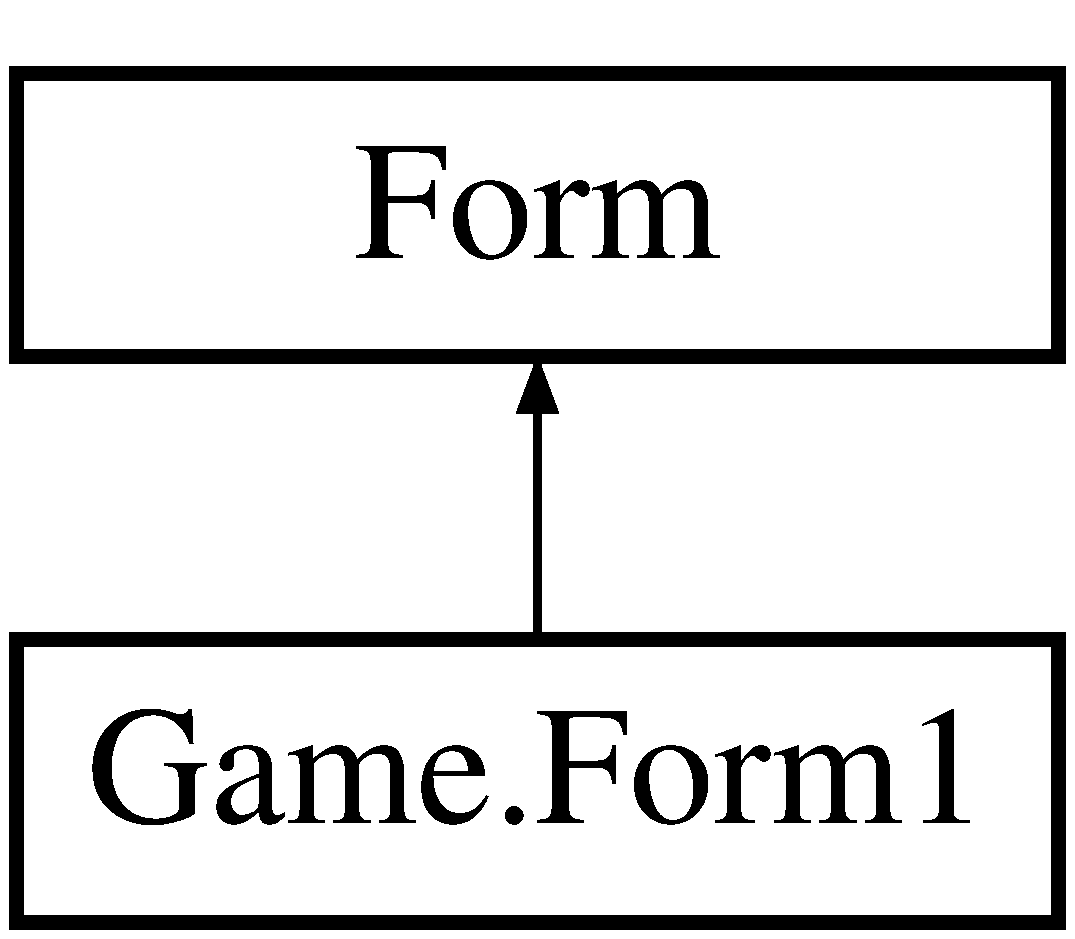
\includegraphics[height=2.000000cm]{class_game_1_1_form1}
\end{center}
\end{figure}
\subsection*{Открытые члены}
\begin{DoxyCompactItemize}
\item 
\hyperlink{class_game_1_1_form1_a6816169b9fcc0021728c2944b192e52c}{Form1} ()
\begin{DoxyCompactList}\small\item\em Инициализация объектов отрисовки, сетки с объектами, текстур и времени \end{DoxyCompactList}\end{DoxyCompactItemize}
\subsection*{Защищенные члены}
\begin{DoxyCompactItemize}
\item 
override void \hyperlink{class_game_1_1_form1_ac06680e001f7a894e19cd07852190ea1}{Dispose} (bool disposing)
\begin{DoxyCompactList}\small\item\em Освободить все используемые ресурсы. \end{DoxyCompactList}\end{DoxyCompactItemize}


\subsection{Подробное описание}
Класс формы, на которой происходит отображение всех объектов 



\subsection{Конструктор(ы)}
\mbox{\Hypertarget{class_game_1_1_form1_a6816169b9fcc0021728c2944b192e52c}\label{class_game_1_1_form1_a6816169b9fcc0021728c2944b192e52c}} 
\index{Game\+::\+Form1@{Game\+::\+Form1}!Form1@{Form1}}
\index{Form1@{Form1}!Game\+::\+Form1@{Game\+::\+Form1}}
\subsubsection{\texorpdfstring{Form1()}{Form1()}}
{\footnotesize\ttfamily Game.\+Form1.\+Form1 (\begin{DoxyParamCaption}{ }\end{DoxyParamCaption})}



Инициализация объектов отрисовки, сетки с объектами, текстур и времени 



\subsection{Методы}
\mbox{\Hypertarget{class_game_1_1_form1_ac06680e001f7a894e19cd07852190ea1}\label{class_game_1_1_form1_ac06680e001f7a894e19cd07852190ea1}} 
\index{Game\+::\+Form1@{Game\+::\+Form1}!Dispose@{Dispose}}
\index{Dispose@{Dispose}!Game\+::\+Form1@{Game\+::\+Form1}}
\subsubsection{\texorpdfstring{Dispose()}{Dispose()}}
{\footnotesize\ttfamily override void Game.\+Form1.\+Dispose (\begin{DoxyParamCaption}\item[{bool}]{disposing }\end{DoxyParamCaption})\hspace{0.3cm}{\ttfamily [protected]}}



Освободить все используемые ресурсы. 


\begin{DoxyParams}{Аргументы}
{\em disposing} & истинно, если управляемый ресурс должен быть удален; иначе ложно.\\
\hline
\end{DoxyParams}


Объявления и описания членов классов находятся в файлах\+:\begin{DoxyCompactItemize}
\item 
Form1.\+cs\item 
Form1.\+Designer.\+cs\end{DoxyCompactItemize}

\hypertarget{class_game_1_1_extension_1_1_game_control}{}\section{Класс Game.\+Extension.\+Game\+Control}
\label{class_game_1_1_extension_1_1_game_control}\index{Game.\+Extension.\+Game\+Control@{Game.\+Extension.\+Game\+Control}}


Класс расширения Алгоритм нахождения кратчайшего расстояния между двумя точками — A$\ast$  


\subsection*{Открытые статические члены}
\begin{DoxyCompactItemize}
\item 
static List$<$ Point $>$ \hyperlink{class_game_1_1_extension_1_1_game_control_a011fc710c60ead3c70da0dd2469fdeaf}{Find\+Path} (\hyperlink{namespace_game_1_1_enums_ab6782702f41f926eb2b923ee03a88069}{Type\+Of\+Cell}\mbox{[},\mbox{]} cells\+Of\+Net, Point start, Point goal, Point Begin\+Net, int scale)
\begin{DoxyCompactList}\small\item\em Основной метод вычисления маршрута, кратчайшего пути \end{DoxyCompactList}\item 
static List$<$ Point $>$ \hyperlink{class_game_1_1_extension_1_1_game_control_a25de72a65a2d4408d800805e7a721e74}{Optimized\+Find\+Path} (List$<$ Point $>$ previous\+Way, \hyperlink{namespace_game_1_1_enums_ab6782702f41f926eb2b923ee03a88069}{Type\+Of\+Cell}\mbox{[},\mbox{]} cells\+Of\+Net, Point start, Point goal, Point Begin\+Net, int scale)
\begin{DoxyCompactList}\small\item\em Основной метод вычисления маршрута, кратчайшего пути \end{DoxyCompactList}\end{DoxyCompactItemize}


\subsection{Подробное описание}
Класс расширения Алгоритм нахождения кратчайшего расстояния между двумя точками — A$\ast$ 



\subsection{Методы}
\mbox{\Hypertarget{class_game_1_1_extension_1_1_game_control_a011fc710c60ead3c70da0dd2469fdeaf}\label{class_game_1_1_extension_1_1_game_control_a011fc710c60ead3c70da0dd2469fdeaf}} 
\index{Game\+::\+Extension\+::\+Game\+Control@{Game\+::\+Extension\+::\+Game\+Control}!Find\+Path@{Find\+Path}}
\index{Find\+Path@{Find\+Path}!Game\+::\+Extension\+::\+Game\+Control@{Game\+::\+Extension\+::\+Game\+Control}}
\subsubsection{\texorpdfstring{Find\+Path()}{FindPath()}}
{\footnotesize\ttfamily static List$<$Point$>$ Game.\+Extension.\+Game\+Control.\+Find\+Path (\begin{DoxyParamCaption}\item[{\hyperlink{namespace_game_1_1_enums_ab6782702f41f926eb2b923ee03a88069}{Type\+Of\+Cell}}]{cells\+Of\+Net\mbox{[},\mbox{]},  }\item[{Point}]{start,  }\item[{Point}]{goal,  }\item[{Point}]{Begin\+Net,  }\item[{int}]{scale }\end{DoxyParamCaption})\hspace{0.3cm}{\ttfamily [static]}}



Основной метод вычисления маршрута, кратчайшего пути 


\begin{DoxyParams}{Аргументы}
{\em cells\+Of\+Net} & Исходная сетка, на которой ищей кратчайший путь\\
\hline
{\em start} & Клетка, от которой начинаем поиск пути\\
\hline
{\em goal} & Клетка, до которой ищем путь\\
\hline
{\em Begin\+Net} & Начальное положение отображаемой сетки\\
\hline
{\em scale} & Масштаб отображаемой области, на которой ищется кратчайший путь\\
\hline
\end{DoxyParams}
\begin{DoxyReturn}{Возвращает}
Возвращает найденный путь, список вершин
\end{DoxyReturn}
\mbox{\Hypertarget{class_game_1_1_extension_1_1_game_control_a25de72a65a2d4408d800805e7a721e74}\label{class_game_1_1_extension_1_1_game_control_a25de72a65a2d4408d800805e7a721e74}} 
\index{Game\+::\+Extension\+::\+Game\+Control@{Game\+::\+Extension\+::\+Game\+Control}!Optimized\+Find\+Path@{Optimized\+Find\+Path}}
\index{Optimized\+Find\+Path@{Optimized\+Find\+Path}!Game\+::\+Extension\+::\+Game\+Control@{Game\+::\+Extension\+::\+Game\+Control}}
\subsubsection{\texorpdfstring{Optimized\+Find\+Path()}{OptimizedFindPath()}}
{\footnotesize\ttfamily static List$<$Point$>$ Game.\+Extension.\+Game\+Control.\+Optimized\+Find\+Path (\begin{DoxyParamCaption}\item[{List$<$ Point $>$}]{previous\+Way,  }\item[{\hyperlink{namespace_game_1_1_enums_ab6782702f41f926eb2b923ee03a88069}{Type\+Of\+Cell}}]{cells\+Of\+Net\mbox{[},\mbox{]},  }\item[{Point}]{start,  }\item[{Point}]{goal,  }\item[{Point}]{Begin\+Net,  }\item[{int}]{scale }\end{DoxyParamCaption})\hspace{0.3cm}{\ttfamily [static]}}



Основной метод вычисления маршрута, кратчайшего пути 


\begin{DoxyParams}{Аргументы}
{\em previous\+Way} & Предыдущий найденный путь\\
\hline
{\em cells\+Of\+Net} & Исходная сетка, на которой ищей кратчайший путь\\
\hline
{\em start} & Клетка, от которой начинаем поиск пути\\
\hline
{\em goal} & Клетка, до которой ищем путь\\
\hline
{\em Begin\+Net} & Начальное положение отображаемой сетки\\
\hline
{\em scale} & Масштаб отображаемой области, на которой ищется кратчайший путь\\
\hline
\end{DoxyParams}
\begin{DoxyReturn}{Возвращает}
Возвращает найденный путь, список вершин
\end{DoxyReturn}


Объявления и описания членов класса находятся в файле\+:\begin{DoxyCompactItemize}
\item 
Extension/Game\+Control.\+cs\end{DoxyCompactItemize}

\hypertarget{class_game_1_1_extension_1_1_game_rendering}{}\section{Класс Game.\+Extension.\+Game\+Rendering}
\label{class_game_1_1_extension_1_1_game_rendering}\index{Game.\+Extension.\+Game\+Rendering@{Game.\+Extension.\+Game\+Rendering}}


Класс расширения Отрисовка объектов  


\subsection*{Открытые статические члены}
\begin{DoxyCompactItemize}
\item 
static void \hyperlink{class_game_1_1_extension_1_1_game_rendering_ab6e8f4d36817459fcb0ee25974c954e8}{Render\+Net} (\hyperlink{class_game_1_1_models_1_1_net}{Net} net, Point first, Simple\+Open\+Gl\+Control Scene, int scale, bool is\+Nigth)
\begin{DoxyCompactList}\small\item\em Отрисовка сетки и ячеек в сетке \end{DoxyCompactList}\item 
static Point \hyperlink{class_game_1_1_extension_1_1_game_rendering_a07669ea2f3fdcc43890d18f79e822c3d}{Graph\+Point\+To\+Algorithm\+Point} (int x, int y)
\begin{DoxyCompactList}\small\item\em Перевод графической точки в точку на алгоритмической сетке \end{DoxyCompactList}\item 
static void \hyperlink{class_game_1_1_extension_1_1_game_rendering_a6ec1beb15590737b78445a193025850b}{Render\+Field} (Simple\+Open\+Gl\+Control Scene, bool is\+Nigth)
\begin{DoxyCompactList}\small\item\em отрисовка поля по всей области \end{DoxyCompactList}\item 
static Point \hyperlink{class_game_1_1_extension_1_1_game_rendering_af6e48165a35d51a6eb41bc4d0ca42843}{Render\+Mouse\+Click\+Graph\+Point} (int x, int y, \hyperlink{namespace_game_1_1_enums_a2d1ea7762a7b4609383b4b578d1c4a60}{Textures} type)
\begin{DoxyCompactList}\small\item\em Отрисовка клетки, куда было произведено нажатие мыши, \end{DoxyCompactList}\item 
static void \hyperlink{class_game_1_1_extension_1_1_game_rendering_af93650c68c4abc9f2c023a62126ed1b8}{Render\+Mouse\+Click\+Algorithm\+Point} (int x, int y, \hyperlink{namespace_game_1_1_enums_a2d1ea7762a7b4609383b4b578d1c4a60}{Textures} type)
\begin{DoxyCompactList}\small\item\em Отрисовка клетки, куда было произведено нажатие мыши, на алгоритмической сетке \end{DoxyCompactList}\item 
static void \hyperlink{class_game_1_1_extension_1_1_game_rendering_a7bffef7924763d901c2890f3dce4c99e}{Render\+Finish\+Square\+Graph\+Point} (Point begin)
\begin{DoxyCompactList}\small\item\em Отрисовка финишной клетки \end{DoxyCompactList}\item 
static void \hyperlink{class_game_1_1_extension_1_1_game_rendering_a23b03c4bb880b092b0834aa5bca2715b}{Render\+Lamp\+And\+Light\+Graph\+Point} (Point begin\+Graph, \hyperlink{namespace_game_1_1_enums_a2d1ea7762a7b4609383b4b578d1c4a60}{Textures} type)
\begin{DoxyCompactList}\small\item\em Отрисовка факела \end{DoxyCompactList}\item 
static void \hyperlink{class_game_1_1_extension_1_1_game_rendering_ab1c58442dbdfc4014074c223980fb528}{Render\+Way\+By\+Algorithm\+Point} (List$<$ Point $>$ way)
\begin{DoxyCompactList}\small\item\em Отрисовка пути через центры ячеек пути \end{DoxyCompactList}\end{DoxyCompactItemize}
\subsection*{Статические открытые данные}
\begin{DoxyCompactItemize}
\item 
static uint \hyperlink{class_game_1_1_extension_1_1_game_rendering_a6c0bd6e66bed4cf38ea83d0542992e04}{m\+Gl\+Texture\+Object0} = 0
\begin{DoxyCompactList}\small\item\em Блок препятствие \end{DoxyCompactList}\item 
static uint \hyperlink{class_game_1_1_extension_1_1_game_rendering_ad6609b7ae66edf828f7b547066efaf5a}{m\+Gl\+Texture\+Object1} = 0
\begin{DoxyCompactList}\small\item\em Прозрачный персонаж \end{DoxyCompactList}\item 
static uint \hyperlink{class_game_1_1_extension_1_1_game_rendering_ab090569badde0919e35aaee6370e206c}{m\+Gl\+Texture\+Object2} = 0
\begin{DoxyCompactList}\small\item\em Текущий персонаж \end{DoxyCompactList}\item 
static uint \hyperlink{class_game_1_1_extension_1_1_game_rendering_a8ec1596e0037600701b755599f6e11be}{m\+Gl\+Texture\+Object3} = 0
\begin{DoxyCompactList}\small\item\em Факел \end{DoxyCompactList}\item 
static uint \hyperlink{class_game_1_1_extension_1_1_game_rendering_accbd80315371256cc927e9b3baadfd6a}{m\+Gl\+Texture\+Object4} = 0
\begin{DoxyCompactList}\small\item\em Трава днем \end{DoxyCompactList}\item 
static uint \hyperlink{class_game_1_1_extension_1_1_game_rendering_a90bbb694accecc307b0898f75b038d57}{m\+Gl\+Texture\+Object5} = 0
\begin{DoxyCompactList}\small\item\em Трава ночью \end{DoxyCompactList}\item 
static bool \hyperlink{class_game_1_1_extension_1_1_game_rendering_a9748f6d2264411c2d27d6ed198defce6}{texture\+Is\+Load} = false
\begin{DoxyCompactList}\small\item\em Загружена ли текстура \end{DoxyCompactList}\end{DoxyCompactItemize}


\subsection{Подробное описание}
Класс расширения Отрисовка объектов 



\subsection{Методы}
\mbox{\Hypertarget{class_game_1_1_extension_1_1_game_rendering_a07669ea2f3fdcc43890d18f79e822c3d}\label{class_game_1_1_extension_1_1_game_rendering_a07669ea2f3fdcc43890d18f79e822c3d}} 
\index{Game\+::\+Extension\+::\+Game\+Rendering@{Game\+::\+Extension\+::\+Game\+Rendering}!Graph\+Point\+To\+Algorithm\+Point@{Graph\+Point\+To\+Algorithm\+Point}}
\index{Graph\+Point\+To\+Algorithm\+Point@{Graph\+Point\+To\+Algorithm\+Point}!Game\+::\+Extension\+::\+Game\+Rendering@{Game\+::\+Extension\+::\+Game\+Rendering}}
\subsubsection{\texorpdfstring{Graph\+Point\+To\+Algorithm\+Point()}{GraphPointToAlgorithmPoint()}}
{\footnotesize\ttfamily static Point Game.\+Extension.\+Game\+Rendering.\+Graph\+Point\+To\+Algorithm\+Point (\begin{DoxyParamCaption}\item[{int}]{x,  }\item[{int}]{y }\end{DoxyParamCaption})\hspace{0.3cm}{\ttfamily [static]}}



Перевод графической точки в точку на алгоритмической сетке 


\begin{DoxyParams}{Аргументы}
{\em x} & Абсцисса точки\\
\hline
{\em y} & Ордината точки\\
\hline
\end{DoxyParams}
\begin{DoxyReturn}{Возвращает}

\end{DoxyReturn}
\mbox{\Hypertarget{class_game_1_1_extension_1_1_game_rendering_a6ec1beb15590737b78445a193025850b}\label{class_game_1_1_extension_1_1_game_rendering_a6ec1beb15590737b78445a193025850b}} 
\index{Game\+::\+Extension\+::\+Game\+Rendering@{Game\+::\+Extension\+::\+Game\+Rendering}!Render\+Field@{Render\+Field}}
\index{Render\+Field@{Render\+Field}!Game\+::\+Extension\+::\+Game\+Rendering@{Game\+::\+Extension\+::\+Game\+Rendering}}
\subsubsection{\texorpdfstring{Render\+Field()}{RenderField()}}
{\footnotesize\ttfamily static void Game.\+Extension.\+Game\+Rendering.\+Render\+Field (\begin{DoxyParamCaption}\item[{Simple\+Open\+Gl\+Control}]{Scene,  }\item[{bool}]{is\+Nigth }\end{DoxyParamCaption})\hspace{0.3cm}{\ttfamily [static]}}



отрисовка поля по всей области 


\begin{DoxyParams}{Аргументы}
{\em Scene} & области отрисовки\\
\hline
{\em is\+Nigth} & текущее время суток (true — ночь, false — день)\\
\hline
\end{DoxyParams}
\mbox{\Hypertarget{class_game_1_1_extension_1_1_game_rendering_a7bffef7924763d901c2890f3dce4c99e}\label{class_game_1_1_extension_1_1_game_rendering_a7bffef7924763d901c2890f3dce4c99e}} 
\index{Game\+::\+Extension\+::\+Game\+Rendering@{Game\+::\+Extension\+::\+Game\+Rendering}!Render\+Finish\+Square\+Graph\+Point@{Render\+Finish\+Square\+Graph\+Point}}
\index{Render\+Finish\+Square\+Graph\+Point@{Render\+Finish\+Square\+Graph\+Point}!Game\+::\+Extension\+::\+Game\+Rendering@{Game\+::\+Extension\+::\+Game\+Rendering}}
\subsubsection{\texorpdfstring{Render\+Finish\+Square\+Graph\+Point()}{RenderFinishSquareGraphPoint()}}
{\footnotesize\ttfamily static void Game.\+Extension.\+Game\+Rendering.\+Render\+Finish\+Square\+Graph\+Point (\begin{DoxyParamCaption}\item[{Point}]{begin }\end{DoxyParamCaption})\hspace{0.3cm}{\ttfamily [static]}}



Отрисовка финишной клетки 


\begin{DoxyParams}{Аргументы}
{\em begin} & Координаты финишной клетки\\
\hline
\end{DoxyParams}
\mbox{\Hypertarget{class_game_1_1_extension_1_1_game_rendering_a23b03c4bb880b092b0834aa5bca2715b}\label{class_game_1_1_extension_1_1_game_rendering_a23b03c4bb880b092b0834aa5bca2715b}} 
\index{Game\+::\+Extension\+::\+Game\+Rendering@{Game\+::\+Extension\+::\+Game\+Rendering}!Render\+Lamp\+And\+Light\+Graph\+Point@{Render\+Lamp\+And\+Light\+Graph\+Point}}
\index{Render\+Lamp\+And\+Light\+Graph\+Point@{Render\+Lamp\+And\+Light\+Graph\+Point}!Game\+::\+Extension\+::\+Game\+Rendering@{Game\+::\+Extension\+::\+Game\+Rendering}}
\subsubsection{\texorpdfstring{Render\+Lamp\+And\+Light\+Graph\+Point()}{RenderLampAndLightGraphPoint()}}
{\footnotesize\ttfamily static void Game.\+Extension.\+Game\+Rendering.\+Render\+Lamp\+And\+Light\+Graph\+Point (\begin{DoxyParamCaption}\item[{Point}]{begin\+Graph,  }\item[{\hyperlink{namespace_game_1_1_enums_a2d1ea7762a7b4609383b4b578d1c4a60}{Textures}}]{type }\end{DoxyParamCaption})\hspace{0.3cm}{\ttfamily [static]}}



Отрисовка факела 


\begin{DoxyParams}{Аргументы}
{\em begin\+Graph} & Начальное положение отрисовки (графические координаты)\\
\hline
{\em type} & Тип отрисовываемой текстуры\\
\hline
\end{DoxyParams}
\mbox{\Hypertarget{class_game_1_1_extension_1_1_game_rendering_af93650c68c4abc9f2c023a62126ed1b8}\label{class_game_1_1_extension_1_1_game_rendering_af93650c68c4abc9f2c023a62126ed1b8}} 
\index{Game\+::\+Extension\+::\+Game\+Rendering@{Game\+::\+Extension\+::\+Game\+Rendering}!Render\+Mouse\+Click\+Algorithm\+Point@{Render\+Mouse\+Click\+Algorithm\+Point}}
\index{Render\+Mouse\+Click\+Algorithm\+Point@{Render\+Mouse\+Click\+Algorithm\+Point}!Game\+::\+Extension\+::\+Game\+Rendering@{Game\+::\+Extension\+::\+Game\+Rendering}}
\subsubsection{\texorpdfstring{Render\+Mouse\+Click\+Algorithm\+Point()}{RenderMouseClickAlgorithmPoint()}}
{\footnotesize\ttfamily static void Game.\+Extension.\+Game\+Rendering.\+Render\+Mouse\+Click\+Algorithm\+Point (\begin{DoxyParamCaption}\item[{int}]{x,  }\item[{int}]{y,  }\item[{\hyperlink{namespace_game_1_1_enums_a2d1ea7762a7b4609383b4b578d1c4a60}{Textures}}]{type }\end{DoxyParamCaption})\hspace{0.3cm}{\ttfamily [static]}}



Отрисовка клетки, куда было произведено нажатие мыши, на алгоритмической сетке 


\begin{DoxyParams}{Аргументы}
{\em x} & Абсцисса точки\\
\hline
{\em y} & Ордината точки\\
\hline
{\em type} & Тип отрисовываемой текстуры\\
\hline
\end{DoxyParams}
\mbox{\Hypertarget{class_game_1_1_extension_1_1_game_rendering_af6e48165a35d51a6eb41bc4d0ca42843}\label{class_game_1_1_extension_1_1_game_rendering_af6e48165a35d51a6eb41bc4d0ca42843}} 
\index{Game\+::\+Extension\+::\+Game\+Rendering@{Game\+::\+Extension\+::\+Game\+Rendering}!Render\+Mouse\+Click\+Graph\+Point@{Render\+Mouse\+Click\+Graph\+Point}}
\index{Render\+Mouse\+Click\+Graph\+Point@{Render\+Mouse\+Click\+Graph\+Point}!Game\+::\+Extension\+::\+Game\+Rendering@{Game\+::\+Extension\+::\+Game\+Rendering}}
\subsubsection{\texorpdfstring{Render\+Mouse\+Click\+Graph\+Point()}{RenderMouseClickGraphPoint()}}
{\footnotesize\ttfamily static Point Game.\+Extension.\+Game\+Rendering.\+Render\+Mouse\+Click\+Graph\+Point (\begin{DoxyParamCaption}\item[{int}]{x,  }\item[{int}]{y,  }\item[{\hyperlink{namespace_game_1_1_enums_a2d1ea7762a7b4609383b4b578d1c4a60}{Textures}}]{type }\end{DoxyParamCaption})\hspace{0.3cm}{\ttfamily [static]}}



Отрисовка клетки, куда было произведено нажатие мыши, 


\begin{DoxyParams}{Аргументы}
{\em x} & Абсцисса точки\\
\hline
{\em y} & Ордината точки\\
\hline
{\em type} & Тип отрисовываемой текстуры\\
\hline
\end{DoxyParams}
\begin{DoxyReturn}{Возвращает}
Возвращается точка на алгоритмической сетки
\end{DoxyReturn}
\mbox{\Hypertarget{class_game_1_1_extension_1_1_game_rendering_ab6e8f4d36817459fcb0ee25974c954e8}\label{class_game_1_1_extension_1_1_game_rendering_ab6e8f4d36817459fcb0ee25974c954e8}} 
\index{Game\+::\+Extension\+::\+Game\+Rendering@{Game\+::\+Extension\+::\+Game\+Rendering}!Render\+Net@{Render\+Net}}
\index{Render\+Net@{Render\+Net}!Game\+::\+Extension\+::\+Game\+Rendering@{Game\+::\+Extension\+::\+Game\+Rendering}}
\subsubsection{\texorpdfstring{Render\+Net()}{RenderNet()}}
{\footnotesize\ttfamily static void Game.\+Extension.\+Game\+Rendering.\+Render\+Net (\begin{DoxyParamCaption}\item[{\hyperlink{class_game_1_1_models_1_1_net}{Net}}]{net,  }\item[{Point}]{first,  }\item[{Simple\+Open\+Gl\+Control}]{Scene,  }\item[{int}]{scale,  }\item[{bool}]{is\+Nigth }\end{DoxyParamCaption})\hspace{0.3cm}{\ttfamily [static]}}



Отрисовка сетки и ячеек в сетке 


\begin{DoxyParams}{Аргументы}
{\em net} & Отрисовываемая сетка\\
\hline
{\em first} & Начальное положение отрисовываемой части сетки\\
\hline
{\em Scene} & Графическая область для отрисовки\\
\hline
{\em scale} & Масштаб сетки\\
\hline
{\em is\+Nigth} & Текущее время суток (true — ночь, false — день)\\
\hline
\end{DoxyParams}
\mbox{\Hypertarget{class_game_1_1_extension_1_1_game_rendering_ab1c58442dbdfc4014074c223980fb528}\label{class_game_1_1_extension_1_1_game_rendering_ab1c58442dbdfc4014074c223980fb528}} 
\index{Game\+::\+Extension\+::\+Game\+Rendering@{Game\+::\+Extension\+::\+Game\+Rendering}!Render\+Way\+By\+Algorithm\+Point@{Render\+Way\+By\+Algorithm\+Point}}
\index{Render\+Way\+By\+Algorithm\+Point@{Render\+Way\+By\+Algorithm\+Point}!Game\+::\+Extension\+::\+Game\+Rendering@{Game\+::\+Extension\+::\+Game\+Rendering}}
\subsubsection{\texorpdfstring{Render\+Way\+By\+Algorithm\+Point()}{RenderWayByAlgorithmPoint()}}
{\footnotesize\ttfamily static void Game.\+Extension.\+Game\+Rendering.\+Render\+Way\+By\+Algorithm\+Point (\begin{DoxyParamCaption}\item[{List$<$ Point $>$}]{way }\end{DoxyParamCaption})\hspace{0.3cm}{\ttfamily [static]}}



Отрисовка пути через центры ячеек пути 


\begin{DoxyParams}{Аргументы}
{\em way} & Путь, который необходимо отрисовать\\
\hline
\end{DoxyParams}


\subsection{Данные класса}
\mbox{\Hypertarget{class_game_1_1_extension_1_1_game_rendering_a6c0bd6e66bed4cf38ea83d0542992e04}\label{class_game_1_1_extension_1_1_game_rendering_a6c0bd6e66bed4cf38ea83d0542992e04}} 
\index{Game\+::\+Extension\+::\+Game\+Rendering@{Game\+::\+Extension\+::\+Game\+Rendering}!m\+Gl\+Texture\+Object0@{m\+Gl\+Texture\+Object0}}
\index{m\+Gl\+Texture\+Object0@{m\+Gl\+Texture\+Object0}!Game\+::\+Extension\+::\+Game\+Rendering@{Game\+::\+Extension\+::\+Game\+Rendering}}
\subsubsection{\texorpdfstring{m\+Gl\+Texture\+Object0}{mGlTextureObject0}}
{\footnotesize\ttfamily uint Game.\+Extension.\+Game\+Rendering.\+m\+Gl\+Texture\+Object0 = 0\hspace{0.3cm}{\ttfamily [static]}}



Блок препятствие 

\mbox{\Hypertarget{class_game_1_1_extension_1_1_game_rendering_ad6609b7ae66edf828f7b547066efaf5a}\label{class_game_1_1_extension_1_1_game_rendering_ad6609b7ae66edf828f7b547066efaf5a}} 
\index{Game\+::\+Extension\+::\+Game\+Rendering@{Game\+::\+Extension\+::\+Game\+Rendering}!m\+Gl\+Texture\+Object1@{m\+Gl\+Texture\+Object1}}
\index{m\+Gl\+Texture\+Object1@{m\+Gl\+Texture\+Object1}!Game\+::\+Extension\+::\+Game\+Rendering@{Game\+::\+Extension\+::\+Game\+Rendering}}
\subsubsection{\texorpdfstring{m\+Gl\+Texture\+Object1}{mGlTextureObject1}}
{\footnotesize\ttfamily uint Game.\+Extension.\+Game\+Rendering.\+m\+Gl\+Texture\+Object1 = 0\hspace{0.3cm}{\ttfamily [static]}}



Прозрачный персонаж 

\mbox{\Hypertarget{class_game_1_1_extension_1_1_game_rendering_ab090569badde0919e35aaee6370e206c}\label{class_game_1_1_extension_1_1_game_rendering_ab090569badde0919e35aaee6370e206c}} 
\index{Game\+::\+Extension\+::\+Game\+Rendering@{Game\+::\+Extension\+::\+Game\+Rendering}!m\+Gl\+Texture\+Object2@{m\+Gl\+Texture\+Object2}}
\index{m\+Gl\+Texture\+Object2@{m\+Gl\+Texture\+Object2}!Game\+::\+Extension\+::\+Game\+Rendering@{Game\+::\+Extension\+::\+Game\+Rendering}}
\subsubsection{\texorpdfstring{m\+Gl\+Texture\+Object2}{mGlTextureObject2}}
{\footnotesize\ttfamily uint Game.\+Extension.\+Game\+Rendering.\+m\+Gl\+Texture\+Object2 = 0\hspace{0.3cm}{\ttfamily [static]}}



Текущий персонаж 

\mbox{\Hypertarget{class_game_1_1_extension_1_1_game_rendering_a8ec1596e0037600701b755599f6e11be}\label{class_game_1_1_extension_1_1_game_rendering_a8ec1596e0037600701b755599f6e11be}} 
\index{Game\+::\+Extension\+::\+Game\+Rendering@{Game\+::\+Extension\+::\+Game\+Rendering}!m\+Gl\+Texture\+Object3@{m\+Gl\+Texture\+Object3}}
\index{m\+Gl\+Texture\+Object3@{m\+Gl\+Texture\+Object3}!Game\+::\+Extension\+::\+Game\+Rendering@{Game\+::\+Extension\+::\+Game\+Rendering}}
\subsubsection{\texorpdfstring{m\+Gl\+Texture\+Object3}{mGlTextureObject3}}
{\footnotesize\ttfamily uint Game.\+Extension.\+Game\+Rendering.\+m\+Gl\+Texture\+Object3 = 0\hspace{0.3cm}{\ttfamily [static]}}



Факел 

\mbox{\Hypertarget{class_game_1_1_extension_1_1_game_rendering_accbd80315371256cc927e9b3baadfd6a}\label{class_game_1_1_extension_1_1_game_rendering_accbd80315371256cc927e9b3baadfd6a}} 
\index{Game\+::\+Extension\+::\+Game\+Rendering@{Game\+::\+Extension\+::\+Game\+Rendering}!m\+Gl\+Texture\+Object4@{m\+Gl\+Texture\+Object4}}
\index{m\+Gl\+Texture\+Object4@{m\+Gl\+Texture\+Object4}!Game\+::\+Extension\+::\+Game\+Rendering@{Game\+::\+Extension\+::\+Game\+Rendering}}
\subsubsection{\texorpdfstring{m\+Gl\+Texture\+Object4}{mGlTextureObject4}}
{\footnotesize\ttfamily uint Game.\+Extension.\+Game\+Rendering.\+m\+Gl\+Texture\+Object4 = 0\hspace{0.3cm}{\ttfamily [static]}}



Трава днем 

\mbox{\Hypertarget{class_game_1_1_extension_1_1_game_rendering_a90bbb694accecc307b0898f75b038d57}\label{class_game_1_1_extension_1_1_game_rendering_a90bbb694accecc307b0898f75b038d57}} 
\index{Game\+::\+Extension\+::\+Game\+Rendering@{Game\+::\+Extension\+::\+Game\+Rendering}!m\+Gl\+Texture\+Object5@{m\+Gl\+Texture\+Object5}}
\index{m\+Gl\+Texture\+Object5@{m\+Gl\+Texture\+Object5}!Game\+::\+Extension\+::\+Game\+Rendering@{Game\+::\+Extension\+::\+Game\+Rendering}}
\subsubsection{\texorpdfstring{m\+Gl\+Texture\+Object5}{mGlTextureObject5}}
{\footnotesize\ttfamily uint Game.\+Extension.\+Game\+Rendering.\+m\+Gl\+Texture\+Object5 = 0\hspace{0.3cm}{\ttfamily [static]}}



Трава ночью 

\mbox{\Hypertarget{class_game_1_1_extension_1_1_game_rendering_a9748f6d2264411c2d27d6ed198defce6}\label{class_game_1_1_extension_1_1_game_rendering_a9748f6d2264411c2d27d6ed198defce6}} 
\index{Game\+::\+Extension\+::\+Game\+Rendering@{Game\+::\+Extension\+::\+Game\+Rendering}!texture\+Is\+Load@{texture\+Is\+Load}}
\index{texture\+Is\+Load@{texture\+Is\+Load}!Game\+::\+Extension\+::\+Game\+Rendering@{Game\+::\+Extension\+::\+Game\+Rendering}}
\subsubsection{\texorpdfstring{texture\+Is\+Load}{textureIsLoad}}
{\footnotesize\ttfamily bool Game.\+Extension.\+Game\+Rendering.\+texture\+Is\+Load = false\hspace{0.3cm}{\ttfamily [static]}}



Загружена ли текстура 



Объявления и описания членов класса находятся в файле\+:\begin{DoxyCompactItemize}
\item 
Extension/Game\+Rendering.\+cs\end{DoxyCompactItemize}

\hypertarget{class_game_1_1_extension_1_1_game_textures}{}\section{Класс Game.\+Extension.\+Game\+Textures}
\label{class_game_1_1_extension_1_1_game_textures}\index{Game.\+Extension.\+Game\+Textures@{Game.\+Extension.\+Game\+Textures}}


Класс расширения Работа с текстурами (загрузка)  


\subsection*{Открытые статические члены}
\begin{DoxyCompactItemize}
\item 
static uint \hyperlink{class_game_1_1_extension_1_1_game_textures_a3c65ea227c8143c391531385e244f0b8}{load\+Image} (string url)
\begin{DoxyCompactList}\small\item\em Загрузка изображения для текстур \end{DoxyCompactList}\item 
static uint \hyperlink{class_game_1_1_extension_1_1_game_textures_af190dd4e218dfd333b1d5ee7a9ce71d0}{Make\+Gl\+Texture} (int Format, Int\+Ptr pixels, int w, int h)
\begin{DoxyCompactList}\small\item\em Связывание текстуры \end{DoxyCompactList}\end{DoxyCompactItemize}


\subsection{Подробное описание}
Класс расширения Работа с текстурами (загрузка) 



\subsection{Методы}
\mbox{\Hypertarget{class_game_1_1_extension_1_1_game_textures_a3c65ea227c8143c391531385e244f0b8}\label{class_game_1_1_extension_1_1_game_textures_a3c65ea227c8143c391531385e244f0b8}} 
\index{Game\+::\+Extension\+::\+Game\+Textures@{Game\+::\+Extension\+::\+Game\+Textures}!load\+Image@{load\+Image}}
\index{load\+Image@{load\+Image}!Game\+::\+Extension\+::\+Game\+Textures@{Game\+::\+Extension\+::\+Game\+Textures}}
\subsubsection{\texorpdfstring{load\+Image()}{loadImage()}}
{\footnotesize\ttfamily static uint Game.\+Extension.\+Game\+Textures.\+load\+Image (\begin{DoxyParamCaption}\item[{string}]{url }\end{DoxyParamCaption})\hspace{0.3cm}{\ttfamily [static]}}



Загрузка изображения для текстур 


\begin{DoxyParams}{Аргументы}
{\em url} & Путь до текстуры\\
\hline
\end{DoxyParams}
\begin{DoxyReturn}{Возвращает}
возвращает данные загруженного для текстуры изображения 
\end{DoxyReturn}
\mbox{\Hypertarget{class_game_1_1_extension_1_1_game_textures_af190dd4e218dfd333b1d5ee7a9ce71d0}\label{class_game_1_1_extension_1_1_game_textures_af190dd4e218dfd333b1d5ee7a9ce71d0}} 
\index{Game\+::\+Extension\+::\+Game\+Textures@{Game\+::\+Extension\+::\+Game\+Textures}!Make\+Gl\+Texture@{Make\+Gl\+Texture}}
\index{Make\+Gl\+Texture@{Make\+Gl\+Texture}!Game\+::\+Extension\+::\+Game\+Textures@{Game\+::\+Extension\+::\+Game\+Textures}}
\subsubsection{\texorpdfstring{Make\+Gl\+Texture()}{MakeGlTexture()}}
{\footnotesize\ttfamily static uint Game.\+Extension.\+Game\+Textures.\+Make\+Gl\+Texture (\begin{DoxyParamCaption}\item[{int}]{Format,  }\item[{Int\+Ptr}]{pixels,  }\item[{int}]{w,  }\item[{int}]{h }\end{DoxyParamCaption})\hspace{0.3cm}{\ttfamily [static]}}



Связывание текстуры 


\begin{DoxyParams}{Аргументы}
{\em Format} & Формат создаваемой текстуры\\
\hline
{\em pixels} & Указатель на данные изображения\\
\hline
{\em w} & Ширина изображения\\
\hline
{\em h} & Высота изображения\\
\hline
\end{DoxyParams}
\begin{DoxyReturn}{Возвращает}
Возвращает связанную текстуру в виде uint
\end{DoxyReturn}


Объявления и описания членов класса находятся в файле\+:\begin{DoxyCompactItemize}
\item 
Extension/Game\+Textures.\+cs\end{DoxyCompactItemize}

\hypertarget{class_game_1_1_models_1_1_net}{}\section{Класс Game.\+Models.\+Net}
\label{class_game_1_1_models_1_1_net}\index{Game.\+Models.\+Net@{Game.\+Models.\+Net}}


Класс сетки, на котоой отображаются объекты  


\subsection*{Открытые члены}
\begin{DoxyCompactItemize}
\item 
\hyperlink{class_game_1_1_models_1_1_net_aa67c03c5f8ad53e819b0b5c2ee6178bd}{Net} ()
\begin{DoxyCompactList}\small\item\em Конструктор сетки, генерирование препятствий \end{DoxyCompactList}\item 
Point \hyperlink{class_game_1_1_models_1_1_net_a8c05bb4cd220b4b8919cc03a48656181}{Begin\+Point\+For\+Centering} (Point current\+Click\+Net, Point begin\+Render\+Net, int scale)
\begin{DoxyCompactList}\small\item\em Перемещение начала отобраемой части сетки \end{DoxyCompactList}\item 
void \hyperlink{class_game_1_1_models_1_1_net_a0ff5fb951d307dcd7b90796bff75fcd9}{Generate\+Global\+Net} (int \hyperlink{class_game_1_1_models_1_1_net_aa7d92ddfdbc6d8e1abe177c1ca81f668}{N})
\begin{DoxyCompactList}\small\item\em Генерирование объектов на сетке \end{DoxyCompactList}\item 
bool \hyperlink{class_game_1_1_models_1_1_net_aca9587ab3eac33b7f6b86cbe5148b870}{Is\+Near\+Lamp} (Point pers)
\begin{DoxyCompactList}\small\item\em Проверка на нахождение около фонаря \end{DoxyCompactList}\item 
bool \hyperlink{class_game_1_1_models_1_1_net_a50459352358d183e0c9dbb57f9a8327d}{Is\+Block} (Point point\+Net)
\begin{DoxyCompactList}\small\item\em Проверка клетки сетки на препятствие \end{DoxyCompactList}\item 
bool \hyperlink{class_game_1_1_models_1_1_net_a025aa070144c06dac4138815c40909ed}{Is\+Free} (Point point\+Net)
\begin{DoxyCompactList}\small\item\em Проверка, свободна ли клетка \end{DoxyCompactList}\item 
bool \hyperlink{class_game_1_1_models_1_1_net_a1a5c1a64772f796f40803bee2f529439}{Is\+Lamp} (Point point\+Net)
\begin{DoxyCompactList}\small\item\em Проверка, является ли клетка факелом \end{DoxyCompactList}\item 
void \hyperlink{class_game_1_1_models_1_1_net_adad1b194504159a34c614c976abfd644}{Lamp} (Point begin\+Net)
\begin{DoxyCompactList}\small\item\em Создает факел в указанной клетке \end{DoxyCompactList}\end{DoxyCompactItemize}
\subsection*{Свойства}
\begin{DoxyCompactItemize}
\item 
\hyperlink{namespace_game_1_1_enums_ab6782702f41f926eb2b923ee03a88069}{Type\+Of\+Cell} \mbox{[},\mbox{]} \hyperlink{class_game_1_1_models_1_1_net_a57c0847ac8fc18813d364fc42cc201dc}{Cells\+Of\+Net}\hspace{0.3cm}{\ttfamily  \mbox{[}get\mbox{]}}
\begin{DoxyCompactList}\small\item\em Сетка \end{DoxyCompactList}\item 
int \hyperlink{class_game_1_1_models_1_1_net_aa7d92ddfdbc6d8e1abe177c1ca81f668}{N}\hspace{0.3cm}{\ttfamily  \mbox{[}get\mbox{]}}
\begin{DoxyCompactList}\small\item\em Размерность сетки \end{DoxyCompactList}\item 
Point \hyperlink{class_game_1_1_models_1_1_net_ab7d957b57aab1da2bcc9475689248bc6}{finish} = 60\hspace{0.3cm}{\ttfamily  \mbox{[}get\mbox{]}}
\begin{DoxyCompactList}\small\item\em Финишная клетка \end{DoxyCompactList}\item 
\hyperlink{namespace_game_1_1_enums_ab6782702f41f926eb2b923ee03a88069}{Type\+Of\+Cell} \hyperlink{class_game_1_1_models_1_1_net_af5051726b673aa124d1d6d394ee94970}{this\mbox{[}int i, int j\mbox{]}}\hspace{0.3cm}{\ttfamily  \mbox{[}get, set\mbox{]}}
\begin{DoxyCompactList}\small\item\em Перегрузка индексатора \end{DoxyCompactList}\end{DoxyCompactItemize}


\subsection{Подробное описание}
Класс сетки, на котоой отображаются объекты 



\subsection{Конструктор(ы)}
\mbox{\Hypertarget{class_game_1_1_models_1_1_net_aa67c03c5f8ad53e819b0b5c2ee6178bd}\label{class_game_1_1_models_1_1_net_aa67c03c5f8ad53e819b0b5c2ee6178bd}} 
\index{Game\+::\+Models\+::\+Net@{Game\+::\+Models\+::\+Net}!Net@{Net}}
\index{Net@{Net}!Game\+::\+Models\+::\+Net@{Game\+::\+Models\+::\+Net}}
\subsubsection{\texorpdfstring{Net()}{Net()}}
{\footnotesize\ttfamily Game.\+Models.\+Net.\+Net (\begin{DoxyParamCaption}{ }\end{DoxyParamCaption})}



Конструктор сетки, генерирование препятствий 



\subsection{Методы}
\mbox{\Hypertarget{class_game_1_1_models_1_1_net_a8c05bb4cd220b4b8919cc03a48656181}\label{class_game_1_1_models_1_1_net_a8c05bb4cd220b4b8919cc03a48656181}} 
\index{Game\+::\+Models\+::\+Net@{Game\+::\+Models\+::\+Net}!Begin\+Point\+For\+Centering@{Begin\+Point\+For\+Centering}}
\index{Begin\+Point\+For\+Centering@{Begin\+Point\+For\+Centering}!Game\+::\+Models\+::\+Net@{Game\+::\+Models\+::\+Net}}
\subsubsection{\texorpdfstring{Begin\+Point\+For\+Centering()}{BeginPointForCentering()}}
{\footnotesize\ttfamily Point Game.\+Models.\+Net.\+Begin\+Point\+For\+Centering (\begin{DoxyParamCaption}\item[{Point}]{current\+Click\+Net,  }\item[{Point}]{begin\+Render\+Net,  }\item[{int}]{scale }\end{DoxyParamCaption})}



Перемещение начала отобраемой части сетки 


\begin{DoxyParams}{Аргументы}
{\em current\+Click\+Net} & Текущая точка\\
\hline
{\em begin\+Render\+Net} & Предыдущая точка начала отображаемой сетки\\
\hline
{\em scale} & Масштаб отображаемой части сетки\\
\hline
\end{DoxyParams}
\begin{DoxyReturn}{Возвращает}
Возвращает точку начала отобраемой части сетки
\end{DoxyReturn}
\mbox{\Hypertarget{class_game_1_1_models_1_1_net_a0ff5fb951d307dcd7b90796bff75fcd9}\label{class_game_1_1_models_1_1_net_a0ff5fb951d307dcd7b90796bff75fcd9}} 
\index{Game\+::\+Models\+::\+Net@{Game\+::\+Models\+::\+Net}!Generate\+Global\+Net@{Generate\+Global\+Net}}
\index{Generate\+Global\+Net@{Generate\+Global\+Net}!Game\+::\+Models\+::\+Net@{Game\+::\+Models\+::\+Net}}
\subsubsection{\texorpdfstring{Generate\+Global\+Net()}{GenerateGlobalNet()}}
{\footnotesize\ttfamily void Game.\+Models.\+Net.\+Generate\+Global\+Net (\begin{DoxyParamCaption}\item[{int}]{N }\end{DoxyParamCaption})}



Генерирование объектов на сетке 


\begin{DoxyParams}{Аргументы}
{\em N} & Размерность сетки\\
\hline
\end{DoxyParams}
\mbox{\Hypertarget{class_game_1_1_models_1_1_net_a50459352358d183e0c9dbb57f9a8327d}\label{class_game_1_1_models_1_1_net_a50459352358d183e0c9dbb57f9a8327d}} 
\index{Game\+::\+Models\+::\+Net@{Game\+::\+Models\+::\+Net}!Is\+Block@{Is\+Block}}
\index{Is\+Block@{Is\+Block}!Game\+::\+Models\+::\+Net@{Game\+::\+Models\+::\+Net}}
\subsubsection{\texorpdfstring{Is\+Block()}{IsBlock()}}
{\footnotesize\ttfamily bool Game.\+Models.\+Net.\+Is\+Block (\begin{DoxyParamCaption}\item[{Point}]{point\+Net }\end{DoxyParamCaption})}



Проверка клетки сетки на препятствие 


\begin{DoxyParams}{Аргументы}
{\em point\+Net} & Проверяемая клетка\\
\hline
\end{DoxyParams}
\begin{DoxyReturn}{Возвращает}
true — если клетка block, иначе false
\end{DoxyReturn}
\mbox{\Hypertarget{class_game_1_1_models_1_1_net_a025aa070144c06dac4138815c40909ed}\label{class_game_1_1_models_1_1_net_a025aa070144c06dac4138815c40909ed}} 
\index{Game\+::\+Models\+::\+Net@{Game\+::\+Models\+::\+Net}!Is\+Free@{Is\+Free}}
\index{Is\+Free@{Is\+Free}!Game\+::\+Models\+::\+Net@{Game\+::\+Models\+::\+Net}}
\subsubsection{\texorpdfstring{Is\+Free()}{IsFree()}}
{\footnotesize\ttfamily bool Game.\+Models.\+Net.\+Is\+Free (\begin{DoxyParamCaption}\item[{Point}]{point\+Net }\end{DoxyParamCaption})}



Проверка, свободна ли клетка 


\begin{DoxyParams}{Аргументы}
{\em point\+Net} & Проверяемая клетка\\
\hline
\end{DoxyParams}
\begin{DoxyReturn}{Возвращает}
true — если клетка свободна, иначе false
\end{DoxyReturn}
\mbox{\Hypertarget{class_game_1_1_models_1_1_net_a1a5c1a64772f796f40803bee2f529439}\label{class_game_1_1_models_1_1_net_a1a5c1a64772f796f40803bee2f529439}} 
\index{Game\+::\+Models\+::\+Net@{Game\+::\+Models\+::\+Net}!Is\+Lamp@{Is\+Lamp}}
\index{Is\+Lamp@{Is\+Lamp}!Game\+::\+Models\+::\+Net@{Game\+::\+Models\+::\+Net}}
\subsubsection{\texorpdfstring{Is\+Lamp()}{IsLamp()}}
{\footnotesize\ttfamily bool Game.\+Models.\+Net.\+Is\+Lamp (\begin{DoxyParamCaption}\item[{Point}]{point\+Net }\end{DoxyParamCaption})}



Проверка, является ли клетка факелом 


\begin{DoxyParams}{Аргументы}
{\em point\+Net} & Проверяемая клетка\\
\hline
\end{DoxyParams}
\begin{DoxyReturn}{Возвращает}
true — если клетка факел, иначе false
\end{DoxyReturn}
\mbox{\Hypertarget{class_game_1_1_models_1_1_net_aca9587ab3eac33b7f6b86cbe5148b870}\label{class_game_1_1_models_1_1_net_aca9587ab3eac33b7f6b86cbe5148b870}} 
\index{Game\+::\+Models\+::\+Net@{Game\+::\+Models\+::\+Net}!Is\+Near\+Lamp@{Is\+Near\+Lamp}}
\index{Is\+Near\+Lamp@{Is\+Near\+Lamp}!Game\+::\+Models\+::\+Net@{Game\+::\+Models\+::\+Net}}
\subsubsection{\texorpdfstring{Is\+Near\+Lamp()}{IsNearLamp()}}
{\footnotesize\ttfamily bool Game.\+Models.\+Net.\+Is\+Near\+Lamp (\begin{DoxyParamCaption}\item[{Point}]{pers }\end{DoxyParamCaption})}



Проверка на нахождение около фонаря 


\begin{DoxyParams}{Аргументы}
{\em pers} & Координаты персонажа на сетке\\
\hline
\end{DoxyParams}
\begin{DoxyReturn}{Возвращает}
true — если персонаж недалеко от сетки, иначе false
\end{DoxyReturn}
\mbox{\Hypertarget{class_game_1_1_models_1_1_net_adad1b194504159a34c614c976abfd644}\label{class_game_1_1_models_1_1_net_adad1b194504159a34c614c976abfd644}} 
\index{Game\+::\+Models\+::\+Net@{Game\+::\+Models\+::\+Net}!Lamp@{Lamp}}
\index{Lamp@{Lamp}!Game\+::\+Models\+::\+Net@{Game\+::\+Models\+::\+Net}}
\subsubsection{\texorpdfstring{Lamp()}{Lamp()}}
{\footnotesize\ttfamily void Game.\+Models.\+Net.\+Lamp (\begin{DoxyParamCaption}\item[{Point}]{begin\+Net }\end{DoxyParamCaption})}



Создает факел в указанной клетке 


\begin{DoxyParams}{Аргументы}
{\em begin\+Net} & Клетка,в которой создается факел\\
\hline
\end{DoxyParams}


\subsection{Полный список свойств}
\mbox{\Hypertarget{class_game_1_1_models_1_1_net_a57c0847ac8fc18813d364fc42cc201dc}\label{class_game_1_1_models_1_1_net_a57c0847ac8fc18813d364fc42cc201dc}} 
\index{Game\+::\+Models\+::\+Net@{Game\+::\+Models\+::\+Net}!Cells\+Of\+Net@{Cells\+Of\+Net}}
\index{Cells\+Of\+Net@{Cells\+Of\+Net}!Game\+::\+Models\+::\+Net@{Game\+::\+Models\+::\+Net}}
\subsubsection{\texorpdfstring{Cells\+Of\+Net}{CellsOfNet}}
{\footnotesize\ttfamily \hyperlink{namespace_game_1_1_enums_ab6782702f41f926eb2b923ee03a88069}{Type\+Of\+Cell} \mbox{[},\mbox{]} Game.\+Models.\+Net.\+Cells\+Of\+Net\hspace{0.3cm}{\ttfamily [get]}}



Сетка 

\mbox{\Hypertarget{class_game_1_1_models_1_1_net_ab7d957b57aab1da2bcc9475689248bc6}\label{class_game_1_1_models_1_1_net_ab7d957b57aab1da2bcc9475689248bc6}} 
\index{Game\+::\+Models\+::\+Net@{Game\+::\+Models\+::\+Net}!finish@{finish}}
\index{finish@{finish}!Game\+::\+Models\+::\+Net@{Game\+::\+Models\+::\+Net}}
\subsubsection{\texorpdfstring{finish}{finish}}
{\footnotesize\ttfamily Point Game.\+Models.\+Net.\+finish = 60\hspace{0.3cm}{\ttfamily [get]}}



Финишная клетка 

\mbox{\Hypertarget{class_game_1_1_models_1_1_net_aa7d92ddfdbc6d8e1abe177c1ca81f668}\label{class_game_1_1_models_1_1_net_aa7d92ddfdbc6d8e1abe177c1ca81f668}} 
\index{Game\+::\+Models\+::\+Net@{Game\+::\+Models\+::\+Net}!N@{N}}
\index{N@{N}!Game\+::\+Models\+::\+Net@{Game\+::\+Models\+::\+Net}}
\subsubsection{\texorpdfstring{N}{N}}
{\footnotesize\ttfamily int Game.\+Models.\+Net.\+N\hspace{0.3cm}{\ttfamily [get]}}



Размерность сетки 

\mbox{\Hypertarget{class_game_1_1_models_1_1_net_af5051726b673aa124d1d6d394ee94970}\label{class_game_1_1_models_1_1_net_af5051726b673aa124d1d6d394ee94970}} 
\index{Game\+::\+Models\+::\+Net@{Game\+::\+Models\+::\+Net}!this\mbox{[}int i, int j\mbox{]}@{this[int i, int j]}}
\index{this\mbox{[}int i, int j\mbox{]}@{this[int i, int j]}!Game\+::\+Models\+::\+Net@{Game\+::\+Models\+::\+Net}}
\subsubsection{\texorpdfstring{this[int i, int j]}{this[int i, int j]}}
{\footnotesize\ttfamily \hyperlink{namespace_game_1_1_enums_ab6782702f41f926eb2b923ee03a88069}{Type\+Of\+Cell} Game.\+Models.\+Net.\+this\mbox{[}int i, int j\mbox{]}\hspace{0.3cm}{\ttfamily [get]}, {\ttfamily [set]}}



Перегрузка индексатора 


\begin{DoxyParams}{Аргументы}
{\em i} & Абсцисса клетки\\
\hline
{\em j} & Ордината клетки\\
\hline
\end{DoxyParams}
\begin{DoxyReturn}{Возвращает}

\end{DoxyReturn}


Объявления и описания членов класса находятся в файле\+:\begin{DoxyCompactItemize}
\item 
Models/Net.\+cs\end{DoxyCompactItemize}

\hypertarget{class_game_1_1_models_1_1_path_node}{}\section{Класс Game.\+Models.\+Path\+Node}
\label{class_game_1_1_models_1_1_path_node}\index{Game.\+Models.\+Path\+Node@{Game.\+Models.\+Path\+Node}}


Структура, используемая в алгоритме A$\ast$  


\subsection*{Свойства}
\begin{DoxyCompactItemize}
\item 
Point \hyperlink{class_game_1_1_models_1_1_path_node_a6cece93479e46b7e12f1cb55a5ed8efc}{Position}\hspace{0.3cm}{\ttfamily  \mbox{[}get, set\mbox{]}}
\begin{DoxyCompactList}\small\item\em Координаты точки на карте. \end{DoxyCompactList}\item 
int \hyperlink{class_game_1_1_models_1_1_path_node_ad0b667e8fc2377ce0c41576cfa382b15}{Path\+Length\+From\+Start}\hspace{0.3cm}{\ttfamily  \mbox{[}get, set\mbox{]}}
\begin{DoxyCompactList}\small\item\em Длина пути от старта (G). \end{DoxyCompactList}\item 
\hyperlink{class_game_1_1_models_1_1_path_node}{Path\+Node} \hyperlink{class_game_1_1_models_1_1_path_node_a08e45c8ce9e42586702501c483b7c947}{Came\+From}\hspace{0.3cm}{\ttfamily  \mbox{[}get, set\mbox{]}}
\begin{DoxyCompactList}\small\item\em Точка, из которой пришли в эту точку. \end{DoxyCompactList}\item 
double \hyperlink{class_game_1_1_models_1_1_path_node_a09eae29bd7b3159ca4cd3c370a1dafa6}{Heuristic\+Estimate\+Path\+Length}\hspace{0.3cm}{\ttfamily  \mbox{[}get, set\mbox{]}}
\begin{DoxyCompactList}\small\item\em Примерное расстояние до цели (H). \end{DoxyCompactList}\item 
double \hyperlink{class_game_1_1_models_1_1_path_node_ac199fbf81d9f45f6b0a2ada32016d4e8}{Estimate\+Full\+Path\+Length}\hspace{0.3cm}{\ttfamily  \mbox{[}get\mbox{]}}
\begin{DoxyCompactList}\small\item\em Ожидаемое полное расстояние до цели (F). \end{DoxyCompactList}\end{DoxyCompactItemize}


\subsection{Подробное описание}
Структура, используемая в алгоритме A$\ast$ 



\subsection{Полный список свойств}
\mbox{\Hypertarget{class_game_1_1_models_1_1_path_node_a08e45c8ce9e42586702501c483b7c947}\label{class_game_1_1_models_1_1_path_node_a08e45c8ce9e42586702501c483b7c947}} 
\index{Game\+::\+Models\+::\+Path\+Node@{Game\+::\+Models\+::\+Path\+Node}!Came\+From@{Came\+From}}
\index{Came\+From@{Came\+From}!Game\+::\+Models\+::\+Path\+Node@{Game\+::\+Models\+::\+Path\+Node}}
\subsubsection{\texorpdfstring{Came\+From}{CameFrom}}
{\footnotesize\ttfamily \hyperlink{class_game_1_1_models_1_1_path_node}{Path\+Node} Game.\+Models.\+Path\+Node.\+Came\+From\hspace{0.3cm}{\ttfamily [get]}, {\ttfamily [set]}}



Точка, из которой пришли в эту точку. 

\mbox{\Hypertarget{class_game_1_1_models_1_1_path_node_ac199fbf81d9f45f6b0a2ada32016d4e8}\label{class_game_1_1_models_1_1_path_node_ac199fbf81d9f45f6b0a2ada32016d4e8}} 
\index{Game\+::\+Models\+::\+Path\+Node@{Game\+::\+Models\+::\+Path\+Node}!Estimate\+Full\+Path\+Length@{Estimate\+Full\+Path\+Length}}
\index{Estimate\+Full\+Path\+Length@{Estimate\+Full\+Path\+Length}!Game\+::\+Models\+::\+Path\+Node@{Game\+::\+Models\+::\+Path\+Node}}
\subsubsection{\texorpdfstring{Estimate\+Full\+Path\+Length}{EstimateFullPathLength}}
{\footnotesize\ttfamily double Game.\+Models.\+Path\+Node.\+Estimate\+Full\+Path\+Length\hspace{0.3cm}{\ttfamily [get]}}



Ожидаемое полное расстояние до цели (F). 

\mbox{\Hypertarget{class_game_1_1_models_1_1_path_node_a09eae29bd7b3159ca4cd3c370a1dafa6}\label{class_game_1_1_models_1_1_path_node_a09eae29bd7b3159ca4cd3c370a1dafa6}} 
\index{Game\+::\+Models\+::\+Path\+Node@{Game\+::\+Models\+::\+Path\+Node}!Heuristic\+Estimate\+Path\+Length@{Heuristic\+Estimate\+Path\+Length}}
\index{Heuristic\+Estimate\+Path\+Length@{Heuristic\+Estimate\+Path\+Length}!Game\+::\+Models\+::\+Path\+Node@{Game\+::\+Models\+::\+Path\+Node}}
\subsubsection{\texorpdfstring{Heuristic\+Estimate\+Path\+Length}{HeuristicEstimatePathLength}}
{\footnotesize\ttfamily double Game.\+Models.\+Path\+Node.\+Heuristic\+Estimate\+Path\+Length\hspace{0.3cm}{\ttfamily [get]}, {\ttfamily [set]}}



Примерное расстояние до цели (H). 

\mbox{\Hypertarget{class_game_1_1_models_1_1_path_node_ad0b667e8fc2377ce0c41576cfa382b15}\label{class_game_1_1_models_1_1_path_node_ad0b667e8fc2377ce0c41576cfa382b15}} 
\index{Game\+::\+Models\+::\+Path\+Node@{Game\+::\+Models\+::\+Path\+Node}!Path\+Length\+From\+Start@{Path\+Length\+From\+Start}}
\index{Path\+Length\+From\+Start@{Path\+Length\+From\+Start}!Game\+::\+Models\+::\+Path\+Node@{Game\+::\+Models\+::\+Path\+Node}}
\subsubsection{\texorpdfstring{Path\+Length\+From\+Start}{PathLengthFromStart}}
{\footnotesize\ttfamily int Game.\+Models.\+Path\+Node.\+Path\+Length\+From\+Start\hspace{0.3cm}{\ttfamily [get]}, {\ttfamily [set]}}



Длина пути от старта (G). 

\mbox{\Hypertarget{class_game_1_1_models_1_1_path_node_a6cece93479e46b7e12f1cb55a5ed8efc}\label{class_game_1_1_models_1_1_path_node_a6cece93479e46b7e12f1cb55a5ed8efc}} 
\index{Game\+::\+Models\+::\+Path\+Node@{Game\+::\+Models\+::\+Path\+Node}!Position@{Position}}
\index{Position@{Position}!Game\+::\+Models\+::\+Path\+Node@{Game\+::\+Models\+::\+Path\+Node}}
\subsubsection{\texorpdfstring{Position}{Position}}
{\footnotesize\ttfamily Point Game.\+Models.\+Path\+Node.\+Position\hspace{0.3cm}{\ttfamily [get]}, {\ttfamily [set]}}



Координаты точки на карте. 



Объявления и описания членов класса находятся в файле\+:\begin{DoxyCompactItemize}
\item 
Models/Path\+Node.\+cs\end{DoxyCompactItemize}

\hypertarget{class_game_1_1_program}{}\section{Класс Game.\+Program}
\label{class_game_1_1_program}\index{Game.\+Program@{Game.\+Program}}


Объявления и описания членов класса находятся в файле\+:\begin{DoxyCompactItemize}
\item 
Program.\+cs\end{DoxyCompactItemize}

\hypertarget{class_game_1_1_extension_1_1_work_with_time}{}\section{Класс Game.\+Extension.\+Work\+With\+Time}
\label{class_game_1_1_extension_1_1_work_with_time}\index{Game.\+Extension.\+Work\+With\+Time@{Game.\+Extension.\+Work\+With\+Time}}


Класс расширения Работа со временем  


\subsection*{Открытые статические члены}
\begin{DoxyCompactItemize}
\item 
static bool \hyperlink{class_game_1_1_extension_1_1_work_with_time_ada6b048bfd14c49efb3d32be4fc27b89}{Is\+Night} (int hour)
\begin{DoxyCompactList}\small\item\em Определяет текущее время суток \end{DoxyCompactList}\item 
static bool \hyperlink{class_game_1_1_extension_1_1_work_with_time_a52617dbfe3480e1fdb61f0fb9a49e5ad}{Times\+Of\+Day} (int hour\+Before, int hour\+After)
\begin{DoxyCompactList}\small\item\em Определяет, сменилось ли время суток \end{DoxyCompactList}\item 
static int \hyperlink{class_game_1_1_extension_1_1_work_with_time_ae37335d8f0245588bd981bd71308a6b6}{Sub\+Total\+Time\+Counting\+For\+Way} (List$<$ Point $>$ way, Date\+Time day\+Time, Point begin\+Render\+Net, \hyperlink{class_game_1_1_models_1_1_net}{Net} net, int day\+Time\+Tick)
\begin{DoxyCompactList}\small\item\em Подсчет времени по пути, пройденным персонажем \end{DoxyCompactList}\end{DoxyCompactItemize}


\subsection{Подробное описание}
Класс расширения Работа со временем 



\subsection{Методы}
\mbox{\Hypertarget{class_game_1_1_extension_1_1_work_with_time_ada6b048bfd14c49efb3d32be4fc27b89}\label{class_game_1_1_extension_1_1_work_with_time_ada6b048bfd14c49efb3d32be4fc27b89}} 
\index{Game\+::\+Extension\+::\+Work\+With\+Time@{Game\+::\+Extension\+::\+Work\+With\+Time}!Is\+Night@{Is\+Night}}
\index{Is\+Night@{Is\+Night}!Game\+::\+Extension\+::\+Work\+With\+Time@{Game\+::\+Extension\+::\+Work\+With\+Time}}
\subsubsection{\texorpdfstring{Is\+Night()}{IsNight()}}
{\footnotesize\ttfamily static bool Game.\+Extension.\+Work\+With\+Time.\+Is\+Night (\begin{DoxyParamCaption}\item[{int}]{hour }\end{DoxyParamCaption})\hspace{0.3cm}{\ttfamily [static]}}



Определяет текущее время суток 


\begin{DoxyParams}{Аргументы}
{\em hour} & Часы, для определения времени суток\\
\hline
\end{DoxyParams}
\begin{DoxyReturn}{Возвращает}
Возвращает true если ночь, день — false
\end{DoxyReturn}
\mbox{\Hypertarget{class_game_1_1_extension_1_1_work_with_time_ae37335d8f0245588bd981bd71308a6b6}\label{class_game_1_1_extension_1_1_work_with_time_ae37335d8f0245588bd981bd71308a6b6}} 
\index{Game\+::\+Extension\+::\+Work\+With\+Time@{Game\+::\+Extension\+::\+Work\+With\+Time}!Sub\+Total\+Time\+Counting\+For\+Way@{Sub\+Total\+Time\+Counting\+For\+Way}}
\index{Sub\+Total\+Time\+Counting\+For\+Way@{Sub\+Total\+Time\+Counting\+For\+Way}!Game\+::\+Extension\+::\+Work\+With\+Time@{Game\+::\+Extension\+::\+Work\+With\+Time}}
\subsubsection{\texorpdfstring{Sub\+Total\+Time\+Counting\+For\+Way()}{SubTotalTimeCountingForWay()}}
{\footnotesize\ttfamily static int Game.\+Extension.\+Work\+With\+Time.\+Sub\+Total\+Time\+Counting\+For\+Way (\begin{DoxyParamCaption}\item[{List$<$ Point $>$}]{way,  }\item[{Date\+Time}]{day\+Time,  }\item[{Point}]{begin\+Render\+Net,  }\item[{\hyperlink{class_game_1_1_models_1_1_net}{Net}}]{net,  }\item[{int}]{day\+Time\+Tick }\end{DoxyParamCaption})\hspace{0.3cm}{\ttfamily [static]}}



Подсчет времени по пути, пройденным персонажем 


\begin{DoxyParams}{Аргументы}
{\em way} & Путь персонажа\\
\hline
{\em day\+Time} & Текущее время суток\\
\hline
{\em begin\+Render\+Net} & \\
\hline
{\em net} & Сетка, по которой передвигается персонаж\\
\hline
{\em day\+Time\+Tick} & Модификатор времени суток\\
\hline
\end{DoxyParams}
\begin{DoxyReturn}{Возвращает}
Возвращает число минут — затраченное персонажем на прохождение данного пути
\end{DoxyReturn}
\mbox{\Hypertarget{class_game_1_1_extension_1_1_work_with_time_a52617dbfe3480e1fdb61f0fb9a49e5ad}\label{class_game_1_1_extension_1_1_work_with_time_a52617dbfe3480e1fdb61f0fb9a49e5ad}} 
\index{Game\+::\+Extension\+::\+Work\+With\+Time@{Game\+::\+Extension\+::\+Work\+With\+Time}!Times\+Of\+Day@{Times\+Of\+Day}}
\index{Times\+Of\+Day@{Times\+Of\+Day}!Game\+::\+Extension\+::\+Work\+With\+Time@{Game\+::\+Extension\+::\+Work\+With\+Time}}
\subsubsection{\texorpdfstring{Times\+Of\+Day()}{TimesOfDay()}}
{\footnotesize\ttfamily static bool Game.\+Extension.\+Work\+With\+Time.\+Times\+Of\+Day (\begin{DoxyParamCaption}\item[{int}]{hour\+Before,  }\item[{int}]{hour\+After }\end{DoxyParamCaption})\hspace{0.3cm}{\ttfamily [static]}}



Определяет, сменилось ли время суток 


\begin{DoxyParams}{Аргументы}
{\em hour\+Before} & Часы до события\\
\hline
{\em hour\+After} & Часы после события\\
\hline
\end{DoxyParams}
\begin{DoxyReturn}{Возвращает}

\end{DoxyReturn}


Объявления и описания членов класса находятся в файле\+:\begin{DoxyCompactItemize}
\item 
Extension/Work\+With\+Time.\+cs\end{DoxyCompactItemize}

%--- End generated contents ---

% Index
\backmatter
\newpage
\phantomsection
\clearemptydoublepage
\addcontentsline{toc}{chapter}{Алфавитный указатель}
\printindex

\end{document}
